%!TEX TS-program = xelatex
%!TEX encoding = UTF-8 Unicode


\documentclass{Dissertate}
\usepackage[english]{babel}
\usepackage{color}
\usepackage{textcomp}
\usepackage{colortbl}
\usepackage[justification=centering]{caption} % centra nella pagina le caption
\usepackage{array}
\usepackage{xcolor}
\usepackage{listings}
\usepackage{siunitx}
\usepackage{pgfplots} % carica anche tikz
% Start of 'ignore natbib' hack
\let\bibhang\relax
\let\citename\relax
\let\bibfont\relax
\let\Citeauthor\relax
\expandafter\let\csname ver@natbib.sty\endcsname\relax
% End of 'ignore natbib' hack
\usepackage[autostyle]{csquotes}
\usepackage[backend=biber, sorting=none]{biblatex}
\addbibresource{references.bib} 
\usepackage{titlesec}
\setcounter{tocdepth}{3}
\setcounter{secnumdepth}{3}

\begin{document}

% Python style for highlighting
\newcommand\pythonstyle{\lstset{
language=Python,
basicstyle=\small,
commentstyle=\color[RGB]{67,156,67},
otherkeywords={self},             % Add keywords here
keywordstyle=\color[RGB]{86,156,214},
emph={MyClass,__init__},          % Custom highlighting
emphstyle=\ttb\color{deepred},    % Custom highlighting style
stringstyle=\color[RGB]{208,134,85},
frame=tb,                         % Any extra options here
showstringspaces=false            % 
}}


% Python environment
\lstnewenvironment{python}[1][]
{
\pythonstyle
\lstset{#1}
}
{}

% Python for external files
\newcommand\pythonexternal[2][]{{
\pythonstyle
\lstinputlisting[#1]{#2}}}

% Python for inline
\newcommand\pythoninline[1]{{\pythonstyle\lstinline!#1!}}


% the front matter
%!TEX root = ../dissertation.tex
% Some details about the dissertation.

\title{A new scope for Open Cognition project: task and motion planning through its Neural-Symbolic Knowledge Store ​}
\author{Michele THIELLA}

%If you have one advisor
\advisor{EMANUELE MENEGATTI}

%If you are coadvised
\coadvisorOne{ENRICO PAGELLO}
\coadvisorOneUniversity{Università di Padova}
\coadvisorTwo{ELISA TOSELLO}
%\maketitle
% \copyrightpage
\frontmatter
\setstretch{\dnormalspacing}
% \abstractpage
%\tableofcontents
% %\authorlist
% \listoffigures
%\dedicationpage
% \acknowledgments

% \doublespacing

% include each chapter...
\setcounter{chapter}{0}  % start chapter numbering at 1
\setcounter{page}{1}
%!TEX root = ../dissertation.tex
\chapter{Introduction}
\label{introduction}

Il recupero e la classificazione di forme 3D sono stati oggetto di una grande quantità di lavori di ricerca che sfruttano sia la rappresentazione globale che i descrittori di forma locale. Un panoramica del campo può essere trovata in \cite{Tangelder2007}, \cite{YulanGuo2014}, \cite{BoYijuan} o guardando le varie edizioni del SHREC 3D Retrieval Contest \cite{ShrecContest}. 

Questo progetto si focalizza sul riconoscimento di gesti delle mani, ambito di notevole interesse dovuto alle sue applicazioni in molti campi diversi come l'interazione uomo-computer, la robotica, i giochi per computer e l'interpretazione automatica della lingua dei segni.
I recenti conseguimenti nel campo della Computer Vision hanno permesso di ottenere un miglioramento notevole in algoritmi di questo tipo. In particolare ci sono stati due avanzamenti chiave:

\begin{itemize}
\item Sviluppo di algoritmi di machine learning più potenti, specialmente tecniche di deep learning.
\item Introduzione di telecamere di profondità, come Time-Of-Flight e Structured-light cameras \cite{DalMutto2012}.
\end{itemize}

La soluzione del problema di classificazione di forme 3D usando dati di immagini e video è sempre stata molto impegnativa, ma lo sviluppo di questi due campi ha permesso, sia di capire meglio il contenuto semantico delle immagini, che di utilizzare approcci basati su informazioni tridimensionali. Ad esempio i dati di profondità che si riescono ad ottenere da queste telecamere contengono una descrizione molto accurata della posa della mano e questo è molto utile per le applicazioni di riconoscimento dei gesti.
Il progetto si basa sullo studio di 5 approcci differenti che combinano diverse architetture della rete e vari tipi di dati di input. Infatti non ci si sofferma solo su dati di profondità ma si utilizzano anche mappe di confidenza e immagini RGB. L'unione di queste informazioni porta ai risultati presentati consultabili nelle tabelle alla fine del Capitolo \textbf{\ref{Risultati sperimentali}}.\\

Questa tesi è composta da una parte introduttiva riguardante le Deep Neural Networks e i suoi algoritmi di ottimizzazione, una parte centrale che illustra il set di dati utilizzato e le sue elaborazioni, successivamente vengono spiegate diverse architetture della Convolutional Neural Network utilizzata per il riconoscimento di 11 gesti differenti, ed infine una parte conclusiva di analisi dei risultati.\\

\begin{comment}
Le reti neurali sono basate su tipi di neuroni artificiali. Il primo di essi venne sviluppato negli anni '50 e '60 ed fu chiamato Perceptron. Oggi, è più comune usare altri modelli di neuroni artificiali, ad esempio quello proposto in questo progetto: il Sigmoid Neuron.
Per capire meglio come funziona un Sigmoid Neuron bisogna però accennare al funzionamento di un Perceptron.
La rappresentazione accetta diversi input binari, x1, x2, … e produce una singola uscita binaria:

\begin{figure}
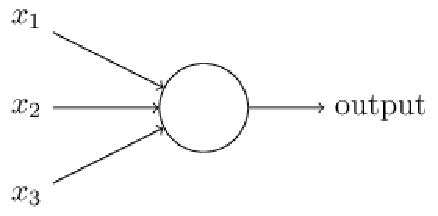
\includegraphics[width=%
0.5\textwidth]{figures/fig01}
\caption[Idea di un perceptron.]{Figura rappresentativa .
\label{fig:myInlineFigure}}
\end{figure}


Nell'esempio mostrato il perceptron ha tre ingressi, x1, x2, x3. In generale potrebbe avere più o meno input. Rosenblatt ha proposto una semplice regola per calcolare l'output. Ha introdotto pesi , w1, w2, … numeri reali che esprimono l'importanza dei rispettivi input per l'output. L'uscita del neurone, 0 o 1, è determinato dal fatto che la somma ponderata ΣjwjXj è minore o maggiore di qualche valore di soglia ( threshold value ). Proprio come i pesi, la soglia è un numero reale che è un parametro del neurone. Per metterlo in termini algebrici più precisi:

$$Output =
\bigg \{
\begin{array}{rl}
0 & \sum_j ( j \, w_j \, X_j ) \le threshold \\
1 & \sum_j ( j \, w_j \, X_j ) > threshold \\
\end{array}
$$

Questo è il modello matematico di base. Un modo in cui puoi pensare al perceptron è che è un dispositivo che prende le decisioni soppesando le prove e da cui, variando i pesi e la soglia, possiamo ottenere diversi modelli di decisione.

Per inciso, quando ho definito i perceptrons ho detto che un perceptron ha solo una singola uscita. Nella rete sopra i perceptron sembrano avere più uscite. In realtà, sono ancora a uscita singola. Le frecce di output multiple sono solo un modo utile per indicare che l'output di un perceptron viene utilizzato come input per molte altre percetron. È meno ingombrante del disegnare una singola linea di uscita che poi si divide.
Semplifichiamo il modo in cui descriviamo i peceptrons.
Il primo cambiamento è scrivere $\sum_j ( j \, w_j \, X_j )$ come prodotto, 
$ w \cdot x \equiv \sum_j ( j \, w_j \, X_j )$, dove w e x sono vettori i cui componenti sono rispettivamente i pesi e gli input. Il secondo cambiamento è spostare la soglia dall'altra parte della disuguaglianza e sostituirla con quella che è nota come bias del perceptron , $b \equiv -threshold$. Usando il bias invece della threshold, la formula del perceptron può essere riscritta:

$$Output =
\bigg \{
\begin{array}{rl}
0 & w\cdot X + b \le 0 \\
1 & w\cdot X + b > 0 \\
\end{array}
$$


Puoi pensare al bias come misura di quanto sia facile far percepire al perceptron un 1. O, per dirla in termini più biologici, la polarizzazione è una misura di quanto sia facile ottenere il perceptron a fuoco . Per un perceptron con una distorsione veramente grande, è estremamente facile per il perceptron emettere un 11. Ma se il bias è molto negativo, allora è difficile per il perceptrone emettere un 1. Ovviamente, introdurre il bias è solo un piccolo cambiamento nel modo in cui descriviamo i percetron, ma vedremo in seguito che questo porta a ulteriori semplificazioni notazionali. Per questo motivo, nel resto del libro non useremo la soglia, useremo sempre il bias.

Tuttavia, la situazione è migliore di quanto suggerisca questa visione. Si scopre che possiamo escogitare algoritmi di apprendimento in grado di sintonizzare automaticamente i pesi e le distorsioni di una rete di neuroni artificiali. Questa sintonizzazione avviene in risposta a stimoli esterni, senza l'intervento diretto di un programmatore.



\newthought{Sigmoid Neuron}

Per vedere come potrebbe funzionare l'apprendimento, supponiamo di fare un piccolo cambiamento in alcuni pesi (o bias) nella rete. Quello che vorremmo è che questo piccolo cambiamento di peso causi solo una piccola variazione corrispondente nell'output dalla rete. Come vedremo tra un momento, questa proprietà renderà possibile l'apprendimento. Schematicamente, ecco cosa vogliamo:

\begin{figure}
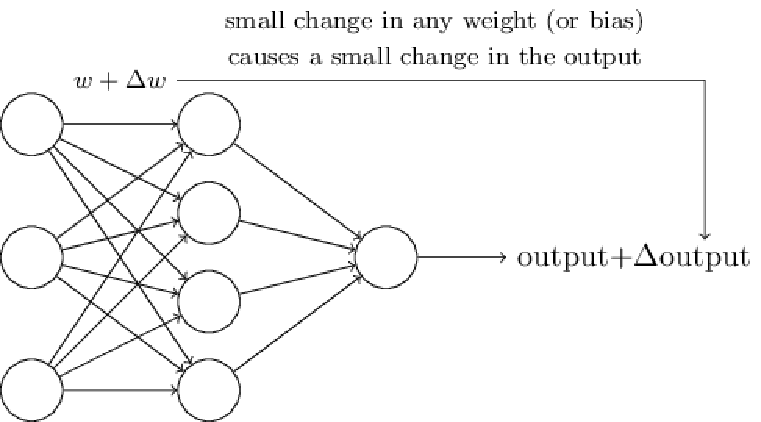
\includegraphics[width=%
0.8\textwidth]{figures/fig08}
\caption[Idea di un s.]{Figura rappresentativa .
\label{fig:myInlineFigure}}
\end{figure}

Se fosse vero che un piccolo cambiamento in un peso (o bias) causa solo un piccolo cambiamento nell'output, allora potremmo usare questo fatto per modificare i pesi e i bias per far sì che la nostra rete si comporti più nel modo che vogliamo. Poi lo ripetiamo, cambiando pesi e bias ripetutamente per produrre risultati migliori e migliori. La rete starebbe imparando.
Il problema è che questo non è ciò che accade quando la nostra rete contiene percetrons. In effetti, un piccolo cambiamento nei pesi o nei bias di ogni singolo perceptron nella rete può a volte far capovolgere completamente l'output di quel perceptron, diciamo da 0 a 1. Questo lancio potrebbe quindi far cambiare completamente il comportamento del resto della rete in un modo molto complicato. 
Ciò rende difficile vedere come modificare gradualmente i pesi e i bias in modo che la rete si avvicini al comportamento desiderato. Forse c'è un modo intelligente per aggirare questo problema. Ma non è immediatamente ovvio come possiamo ottenere una rete di percetrons da imparare.
Possiamo superare questo problema introducendo un nuovo tipo di neurone artificiale chiamato sigmoid neuron . I sigmoid neurons sono simili ai perceptrons, ma modificati in modo che piccoli cambiamenti nei loro pesi e bias causino solo un piccolo cambiamento nella loro produzione. Questo è il fatto cruciale che permetterà a una rete di sigmoid neurons di imparare. 
Descriveremo i sigmoid neurons nello stesso modo in cui abbiamo rappresentato i perceptrons:

Proprio come un perceptron, il sigmoid neuron ha input, x1, x2, … Ma invece di essere solo 0 o 1, questi input possono anche assumere qualsiasi valore compreso tra 0 e 1. Quindi, ad esempio, 0.638... è un input valido per un sigmoid neuron. Inoltre, proprio come un perceptron, il sigmoid neuron ha pesi per ogni input, w1, w2, … e un bias complessivo. Ma l'output non è 0 o 1. 
Invece, è σ ( w ⋅ x + b ), dove σ è chiamata la funzione sigmoide (sigmoid function) ed è definito da:\\

\begin{eqnarray} 
\sigma(z) \equiv \frac{1}{1 + e^{-z}}
\end{eqnarray}

Per dirla in modo un po' più esplicito, l'output di un sigmoid neuron con ingressi x1, x2, …, pesi w1, w2, … e bias b è : \\
\begin{eqnarray} 
\sigma(z) \equiv \frac{1}{1+\exp(-\sum_j w_j x_j-b)}
\end{eqnarray}


A prima vista, i sigmoid neurons appaiono molto diversi dai perceptrons. La forma algebrica della funzione sigmoide può sembrare opaca e proibitiva se non la conosci già. In effetti, ci sono molte somiglianze tra i perceptrons e i sigmoid neurons e la forma algebrica della funzione sigmoide risulta essere più un dettaglio tecnico che una vera barriera alla comprensione.
Per capire la somiglianza con il modello perceptron, supponiamo che 
$z \equiv  w \cdot x + b$ sia un grande numero positivo. Quindi $e^{-z} \approx 0$ e così $\sigma(z) \approx 1$.
In altre parole, quando $z= w \cdot x + b$ è grande e positivo, l'uscita dal sigmoid neuron è di circa 1, proprio come sarebbe stato per un perceptron. Supponiamo d'altra parte che $z = w \cdot x + b$ è molto negativo. Quindi $e^{-z} \to \infty$ e $\sigma(z) \approx 0$. Quindi, quando$ z= w \cdot x + b$ è molto negativo, anche il comportamento di un sigmoid neuron si avvicina molto a un perceptrons. È solo quando $z = w \cdot x + b$ è di dimensioni modeste che c'è molta deviazione dal modello perceptron.
Che dire della forma algebrica di $\sigma$? Come possiamo capirlo? In effetti, la forma esatta di σ non è così importante - ciò che conta davvero è la forma della funzione quando è tracciata. Ecco la forma:

\begin{figure}
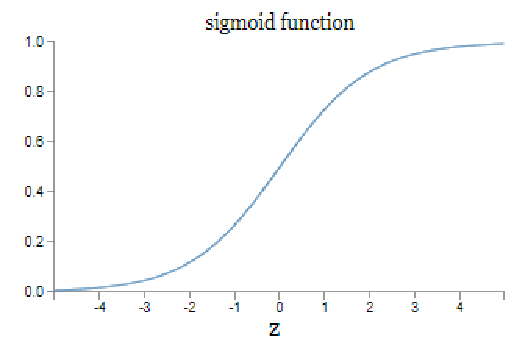
\includegraphics[width=%
0.8\textwidth]{figures/fig10}
\caption[Sigmoid function.]{Figura rappresentativa .
\label{fig:myInlineFigure}}
\end{figure}

Questa forma è una versione attenuata di una funzione di passaggio:

\begin{figure}
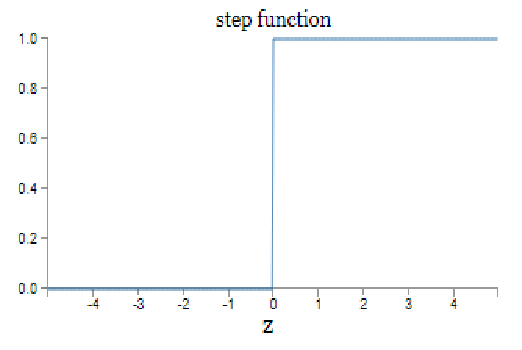
\includegraphics[width=%
0.8\textwidth]{figures/fig11}
\caption[Step function.]{Figura rappresentativa .
\label{fig:myInlineFigure}}
\end{figure}

Se σ era in effetti una funzione a gradino, allora il sigmoide sarebbe stato un perceptron, poiché l'output sarebbe 1 o 0 a seconda che w⋅x+b era positivo o negativo * . Usando il σ attuale la funzione che otteniamo, come già implicato sopra, è una percezione distorta. In effetti, è la scorrevolezza della funzione σ che è il fatto cruciale, non la sua forma dettagliata. La scorrevolezza di σ significa che piccoli cambiamenti Δwj nei pesi e Δb nel bias produrrà un piccolo cambiamento Δoutput nell'output dal neurone. In realtà, il calcolo ci dice che l' Δoutput è ben approssimato da

\begin{eqnarray} 
  \Delta \mbox{output} \approx \sum_j \frac{\partial \, \mbox{output}}{\partial w_j}
  \Delta w_j + \frac{\partial \, \mbox{output}}{\partial b} \Delta b
\end{eqnarray}


dove la somma è sopra tutti i pesi, $w_j$, e $\frac{\partial \, \mbox{output}}{\partial w_j}$ e $\frac{\partial \, \mbox{output}}{\partial b}$ denotano derivate parziali dell'output rispetto a $w_j$ e b, rispettivamente.
Mentre l'espressione sopra sembra complicata, con tutte le derivate parziali, in realtà sta dicendo qualcosa di molto semplice (e che è una buona notizia):

Δoutput è una funzione lineare dei cambiamenti $\Delta w_j$ e $\Delta b$ nei pesi e nei bias. Questa linearità semplifica la scelta di piccoli cambiamenti nei pesi e nei bias per ottenere qualsiasi piccola variazione desiderata nell'output. Quindi, mentre i sigmoid neurons hanno lo stesso comportamento qualitativo di perceptrons, rendono molto più facile capire come il cambiamento dei pesi e dei bias modificherà l'output.

Se è la forma di $\sigma$ che conta davvero, e non la sua forma esatta, allora perché usare la particolare forma usata per $\sigma$ in Equazione (2.1) ? In seguito calcolando le derivate parziali dell'Equazione (2.3), usando $\sigma$ semplificherà l'algebra. In ogni caso, $\sigma$ è comunemente usato nel lavoro sulle reti neurali, ed è la funzione di attivazione che useremo più spesso in questo libro.
Come dovremmo interpretare l'output di un sigmoid neuron? Ovviamente, una grande differenza tra perceptrons e sigmoid neurons è che i sigmoid neurons non producono solo 0 o 1. Possono avere come risultato qualsiasi numero reale tra 0 e 1, quindi valori come 0.173... e 0.689... sono uscite legittime. Questo può essere utile, per esempio, se vogliamo usare il valore di uscita per rappresentare l'intensità media dei pixel in un ingresso di immagine in una rete neurale. Ma a volte può essere una seccatura. Supponiamo di volere l'output dalla rete per indicare "l'immagine di input è un 9" o "l'immagine di input non è un 9". Ovviamente, sarebbe più semplice farlo se l'output fosse uno 0 o un 1, come in un perceptron. Ma in pratica possiamo stabilire una convenzione per affrontarla, ad esempio, decidendo di interpretare qualsiasi output di almeno 0,5 come indica un "9" e qualsiasi uscita inferiore a 0,5 come indicante "non un 9". Indicherò sempre esplicitamente quando usiamo tale convenzione, quindi non dovrebbe causare alcuna confusione.

% For an example of a full page figure, see Fig.~\textbf{\ref{fig:myFullPageFigure}.

%% Requires fltpage2 package
%%
% \begin{FPfigure}
% 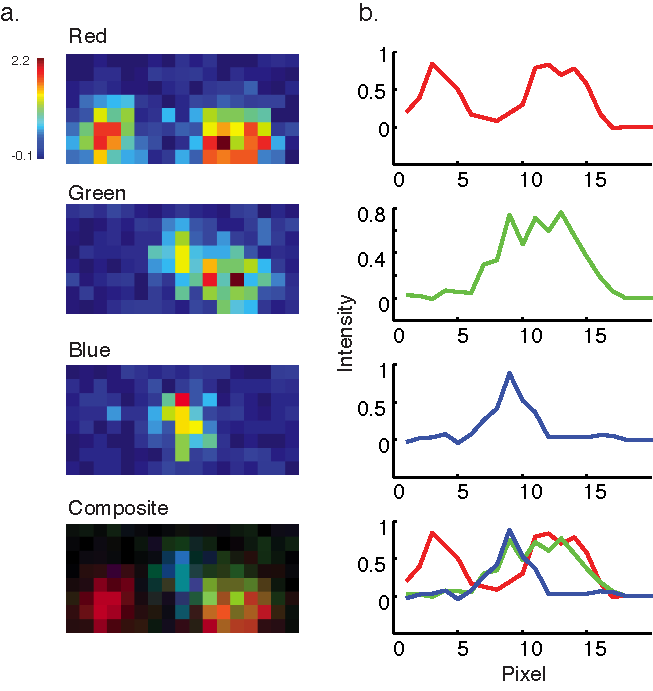
\includegraphics[width=\textwidth]{figures/fullpage}
%\caption[Short figure name.]{This is a full page figure using the FPfigure command. It takes up the whole page and the caption appears on the preceding page. Its useful for large figures. Harvard's rules about full page figures are tricky, but you don't have to worry about it because we took care of it for you. For example, the full figure is supposed to have a title in the same style as the caption but without the actual caption. The caption is supposed to appear alone on the preceding page with no other text. You do't have to worry about any of that. We have modified the fltpage package to make it work. This is a lengthy caption and it clearly would not fit on the same page as the figure. Note that you should only use the FPfigure command in instances where the figure really is too large. If the figure is small enough to fit by the caption than it does not produce the desired effect. Good luck with your thesis. I have to keep writing this to make the caption really long. LaTex is a lot of fun. You will enjoy working with it. Good luck on your post doctoral life! I am looking forward to mine. \label{fig:myFullPageFigure}}
 %\end{FPfigure}
 %\afterpage{\clearpage}
\end{comment}

%!TEX root = ../dissertation.tex
\chapter{OpenCog System} \label{cha:opencog_system}

The OpenCog design aims to capture the spirit of the architecture and dynamics of the brain without imitating the details (which are largely unknown) via:
\begin{itemize}
	\item Integrating together a carefully selected combination of cognitive algorithms acting on different kinds of knowledge.
	\item A scalable, robust and flexible C++ software architecture.
	\item A manner specifically designed:
	\begin{itemize}	
	\item To cooperate together with “cognitive synergy” for the scope of tasks characteristic of human intelligence. 
	\item To give rise to the emergence of an effectively functioning knowledge network in the AI system’s mind, as it interacts with the world, including a self-updating hierarchical/heterarchical ontology and models of itself and others.
	\end{itemize}
\end{itemize}
Following section, Section \ref{sec:cognitive_synergy}, elaborates on the new concepts introduced in these points.


\section{Cognitive Synergy}\label{sec:cognitive_synergy}  %% slide 4 tua presentazione, magari aggiungi le parte in basso

OpenCog is a diverse assemblage of cognitive algorithms, each embodying its own innovations. The power of the overall architecture is its careful adherence to the principle of Cognitive Synergy. \\
The human brain consists of a host of subsystems that perform particular tasks, both specialized and general in nature, connected together in a manner enabling them to synergetically assist, rather than work against each other. \\
The essential principles of Cognitive Synergy Theory (CST) can be summarized in the following points, further explored in \cite{inproceedings_cognitive_synergy}:

\begin{enumerate}
	\item Intelligence can be understood as the ability to achieve complex goals in a certain set of environments. 
	\item An intelligent system requires a \enquote{multi-memory} architecture, meaning the possession of a number of specialized yet interconnected knowledge types.
	\item \enquote{Cognitive processes}: a system must possess knowledge creation mechanisms corresponding to each of these memory types.
	\item Each cognitive process must have the ability to recognize when it lacks information and thus, draw it from knowledge creation mechanisms related to other types of knowledge.
	\item The Cognitive Synergy is, therefore, represented by the interaction between the knowledge creation mechanisms, which perform much more effectively in combination than non-interactive mode. 
	\item The activity of the different cognitive processes involved in an intelligent system can be modeled in terms of the schematic implication \enquote{Context \& Procedure $\rightarrow$ Goal}.
\end{enumerate}

These points are implicit in the systems theory of mind given in \cite{goertzel2006the}, where more thorough characterizations of these ideas can be found.\\
Interactions as mentioned in Points 4 and 5 are the conceptual core of CST. \\
Most AI algorithms suffer from combinatorial explosions. In a “general intelligence” context, there is a lack of intrinsic constraint; consequently, the algorithms are unable to filter through all the possibilities (as opposed to a ANI problem like chessplaying, where the context is huge but constrained and hence restricts the scope of possible combinations that needs to be considered). \\
To decrease the severity of combinatorial explosions, one can use an AGI architecture based on CST, in which the different learning mechanisms dealing with a certain sort of knowledge, are designed to synergize with ones dealing with other sorts of knowledge. \\
It is necessary that each learning mechanism recognizes when it is \enquote{blocked} and then, it can ask for help to the other complementary cognitive mechanisms. \\
The Figure \ref{fig:cognitive_processes} is proposed to give a general visual idea of these concepts. It shows an overview of the most important cognitive dynamics considered in Cognitive Synergy Theory and describes the behavior of a system as it pursues a set of goals, which are then refined by inference (through a logic engine or as an emergent process resulting from the dynamics of an Neural Network system), aided by other processes. \\


\begin{figure} [h]
\centering
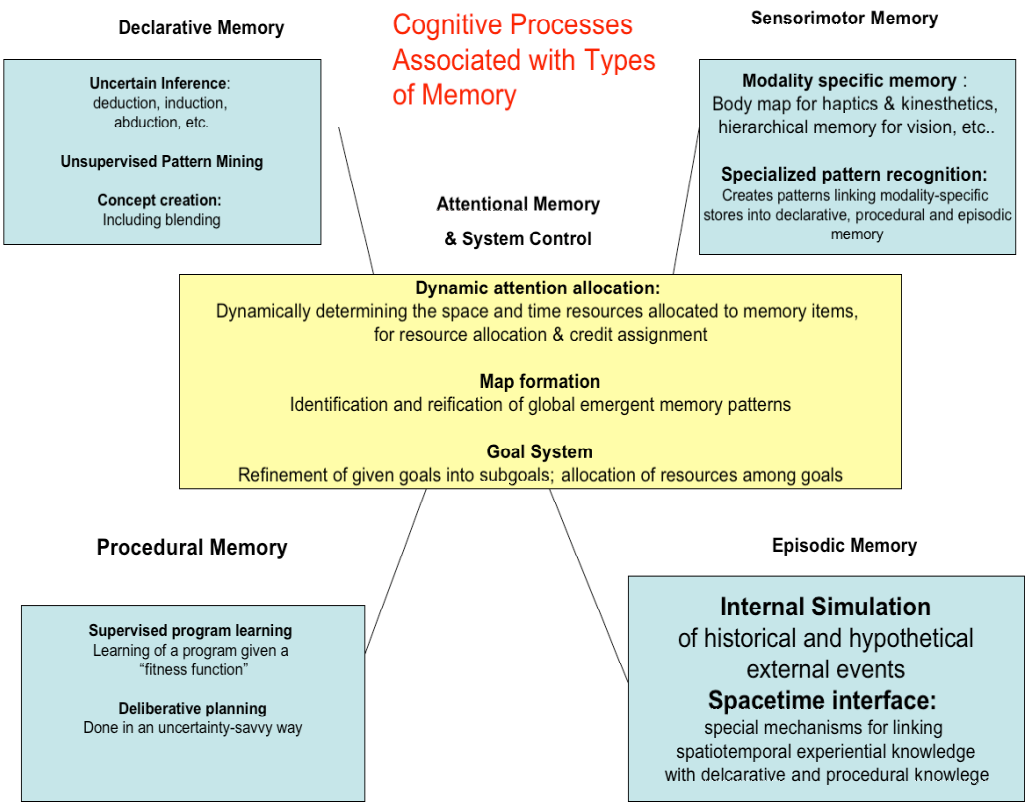
\includegraphics[width=0.7
\textwidth]{figures/Magistrale/04 - cognitive_processes_and_memory}
\caption[Cognitive Processes.]{A high-level overview of the main types of cognitive process considered in Cognitive Synergy Theory, categorized according to the type of knowledge with which each process deals.
\label{fig:cognitive_processes}}
\end{figure} 

The detailed argument explaining how the cognitive algorithm selection and integration methods, chosen by the OpenCog team, will have the desired effect, is sketched on the OpenCog wiki site\footnotemark{} and various previously-published conference papers. It has been presented more thoroughly in the 2014 books Engineering General Intelligence vol. 1 and 2 \cite{DBLP:series/atlantis/GoertzelPG14, DBLP:series/atlantis/GoertzelPG14a}.
\footnotetext{\url{https://wiki.opencog.org/w/Background_Publications}}

\section{OpenCog Architecture}\label{sec:opencog_architecture}

There are several components that make up the basic architecture of OpenCog. In the following sections, they will be described, more or less independently, before being concatenated and contextualized into the problem considered in this project. \\
Currently, the OpenCog project is under strong development and some of the concepts presented here may be obsolete, improved or evolved, or being redesigned. However, much of the basic infrastructure and theory remains unchanged.  

\subsection{Atomspace}\label{sec:atomspace}

The AtomSpace is a platform for building Artificial General Intelligence (AGI) systems. It provides the central knowledge representation component for OpenCog. As such, it is a fairly mature component, on which a lot of other systems are built, and which depend on it for stable, correct operation in a day-to-day production environment. \\
It is a mashup of a large variety of concepts from mathematical logic, theorem proving, graph theory, database theory, type theory, model theory and knowledge representation. \\
More specifically, the OpenCog AtomSpace is an in-RAM knowledge representation database, an associated query engine and graph-re-writing system, and a rule-driven inferencing engine that can apply and manipulate sequences of rules to perform reasoning. \\
The best way to capture all of this, is a kind of in-RAM Generalized Hypergraph (Metagraph) Database. \\
On top of this, the Atomspace provides a variety of advanced features not available anywhere else. It is currently used to store natural language grammars, dictionaries and parsers, to store biochemical and biomedical data, robot control algorithms, machine learning algorithms, audio/video processing pipelines and deep learning neural networks.\\

\subsubsection{Metagraph: a Generalized Hypergraph}\label{sec:gen_hypergraph}

Formally, a graph is:
\begin{itemize}
	\item A set of vertexes $V=\left\{v_{1}, v_{2}, \cdots, v_{M}\right\}$
	\item A set of edges $E=\left\{e_{1}, e_{2}, \cdots, e_{N}\right\}$ where each edge $e_{k}$ is an ordered pair of vertexes drawn from the set $V$.
\end{itemize}
Since edges are ordered pairs, it is conventional to denote them with arrows. In practice, one wishes to associate a label to each vertex, and also some additional attribute data (e.g. weight); likewise for the edges. \\

A hypergraph is very similar to a graph, except for the edges. 
\enquote{Hyperedges} are defined as edges that can contain more than two vertices. That is, the hyperedge, rather than being an ordered pair of vertices, is an ordered list of vertices. \\
Formally, a hypergraph is:
\begin{itemize}
	\item A set of vertexes $V=\left\{v_{1}, v_{2}, \cdots, v_{M}\right\}$
	\item A set of hyperedges $E=\left\{e_{1}, e_{2}, \cdots, e_{N}\right\}$ where each hyperedge $e_{k}$ is an ordered list of vertexes drawn from the set $V$. This list may be empty, or have one, or two, or more members.
\end{itemize}

A good representation of a hypergraph is the one proposed in Figure \ref{fig:atomspace_table}. 
It was a straight-forward extension of the edge table, to which a new column was added for each position and then, those columns were mashed together into one set.  

\begin{figure} [h]
\centering
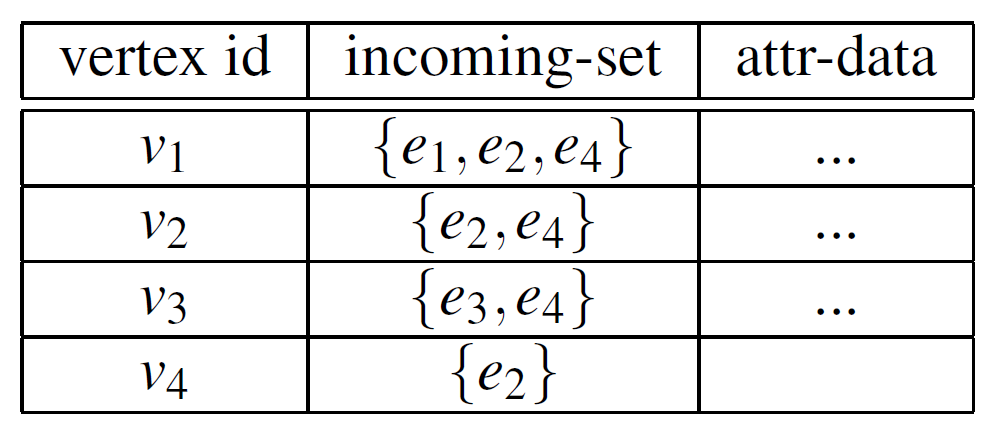
\includegraphics[width=0.7
\textwidth]{figures/Magistrale/atomspace_table}
\caption[Hypergraph edge table]{Hypergraph edge table
\label{fig:atomspace_table}}
\end{figure}

The vertex table looks like the edge table, but the vertex-list is an ordered list, while the incoming-set (the edge-set) really is a set. This is because a hypergraph is “almost” a bipartite graph, having the form of Figure \ref{fig:hypergraph_graph}, with the set E on the left being the set of hyperedges. \\

\begin{figure} [h]
\centering
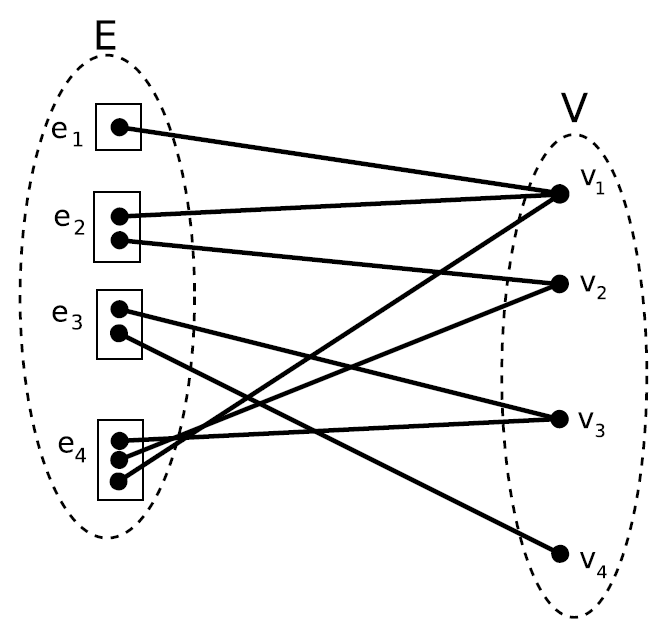
\includegraphics[width=0.6
\textwidth]{figures/Magistrale/hypergraph_graph}
\caption[Hypergraph as bipartite graph]{The $E$ and $V$ ellipses are the hyperedge and vertex tables. The boxes mean that the hyperedges are ordered lists.
\label{fig:hypergraph_graph}}
\end{figure}

Before define a Metagraph, a change of terminology is useful: the basic objects are now called \enquote{Nodes} and \enquote{Links} instead of \enquote{vertexes} and \enquote{edges}. \\
Thus, a Metagraph is:
\begin{itemize}
	\item A set of nodes $V=\left\{v_{1}, v_{2}, \cdots, v_{M}\right\}$
	\item A set of links $E=\left\{e_{1}, e_{2}, \cdots, e_{N}\right\}$ where each hyperedge $e_{k}$ is an ordered list of nodes, or other links, or a mixture. They are arranged to be acyclic (to form a directed acyclic graph).
\end{itemize}

The metagraph is a generalization of a hypergraph, in the sense that now a hyperedge (link) may contain either another vertex (node) or another link. Visually, it has the shape of a Directed Acyclic Graph (DAG), such as the one shown in Figure \ref{fig:metagraph_graph}.

\begin{figure} [h]
\centering
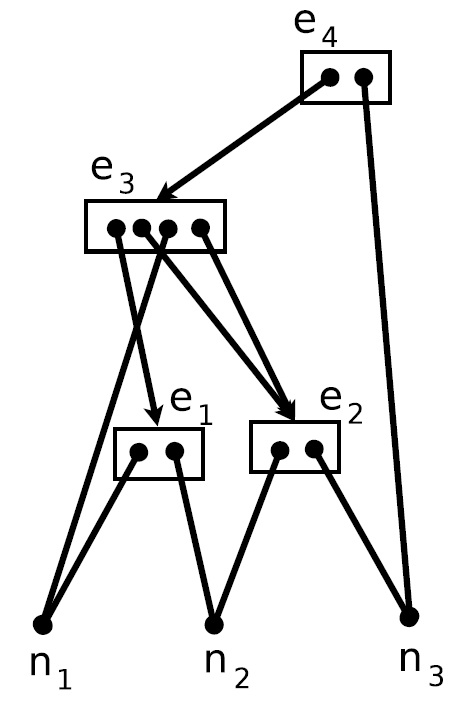
\includegraphics[width=0.4
\textwidth]{figures/Magistrale/metagraph_graph}
\caption[Directed Acyclic Graph ]{An example of a DAG.
\label{fig:metagraph_graph}}
\end{figure}

But in Metagraph, links are ordered lists, represented as boxes. Thus, to convert it in a DAG it is possible to collapse the boxes to single points or to dissolve the boxes entirely and replace a single arrow, from point-to-box, by many arrows, from point to each of the box elements.  \\
Whereas the node table is the same as the vertex table for the hypergraph, nevertheless the link table now requires both an outgoing-atom list and an incoming-link set.
Figure \ref{fig:metagraph_table} shows the result.

\begin{figure} [h]
\centering
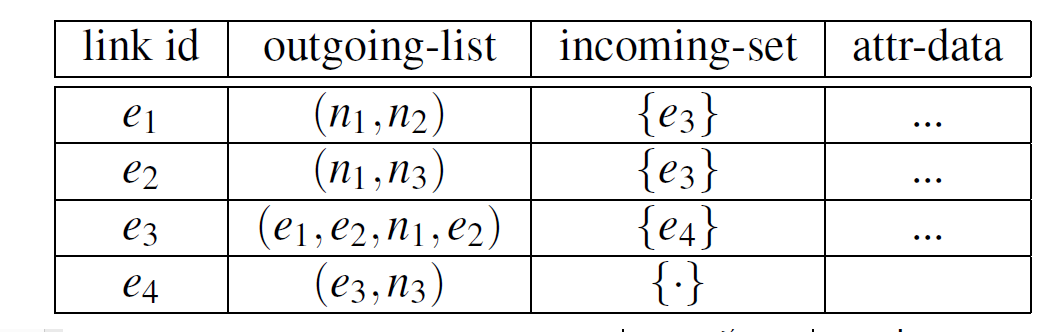
\includegraphics[width=0.8
\textwidth]{figures/Magistrale/metagraph_table}
\caption[Metagraph link table]{Metagraph link table
\label{fig:metagraph_table}}
\end{figure}

For convenience, the name \enquote{Atom} is given to something that is either a node or a link. Links are then, sets of atoms. \\
These concepts are described in \cite{Vep20a, metagraph_app}, where RAM-usage considerations, reasons why metagraphs offer more efficient, more flexible and more powerful ways of representing graphs and reasons why a metagraph store is better than a graph store and much more, can also be found. \\

Finally, some extensions of the metagraph are considered: Typed Metagraph (TMG) and Directed Typed Metagraph (DTMG). \\
Typed metagraphs are defined as hypergraphs with types assigned to hyperedges and their targets, and the potential to have targets of hyperedges connect to whole links, as well as targets. 
An example can be found in Figure \ref{fig:typed_edge}. \\

\begin{figure}[h]
\centering
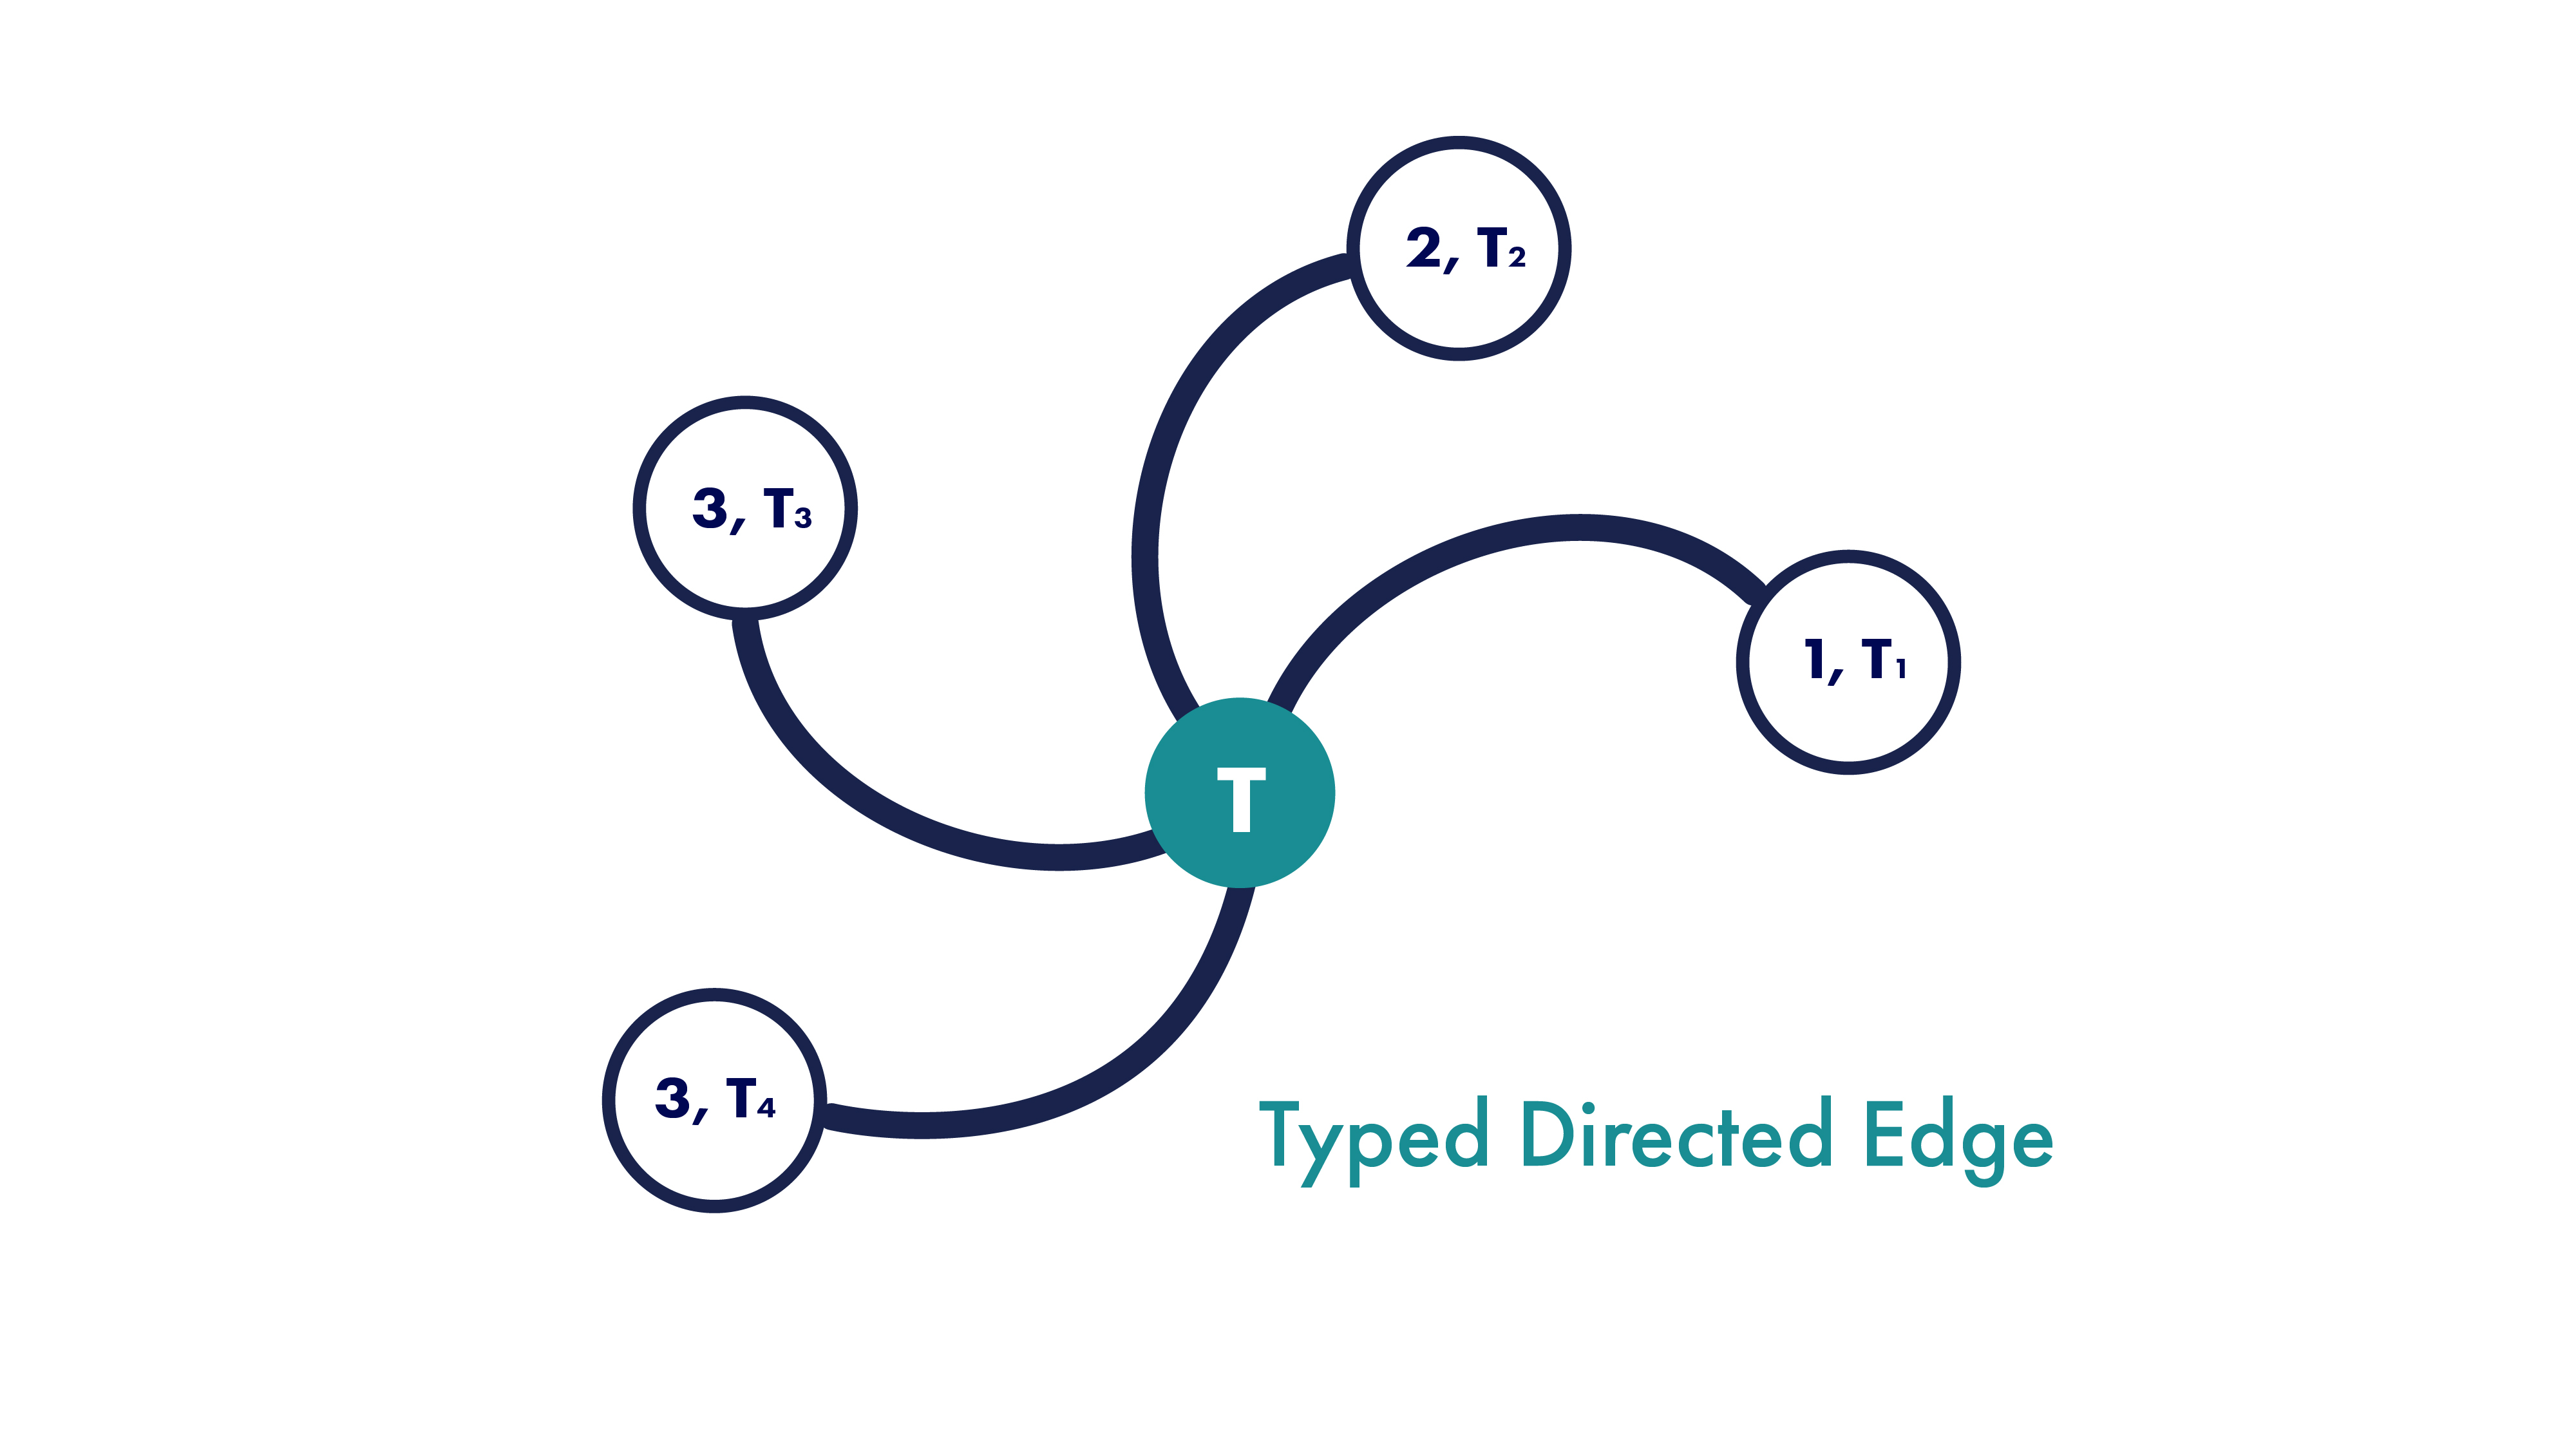
\includegraphics[width=0.6
\textwidth]{figures/Magistrale/typed_edge}
\caption[Typed Directed Edge]{Example of a typed, directed edge. This one has 4 targets. $T$ is the type of the edge itself. The third and fourth targets are unordered relative to each other.
\label{fig:typed_edge}}
\end{figure}

A natural extension of a TMG is the Probabilistically TMG, based on probabilistic dependent types. Thus, one can assign a probability (or an entire probability distribution) to each connection between edges, thanks to the probabilistic type inheritance relations. In this way, it is possible to obtain a KB that can work with probabilistic logic, fuzzy logic, make uncertain inferences and much more. \\
Atomic Directed Typed Metagraphs (atomic DTMG) are introduced via partitioning the targets of each edge in a typed metagraph into input, output and lateral sets; one can then look at \enquote{metapaths} in which edges' output-sets are linked to other edges' input-sets (Figure \ref{fig:typed_metapath}). Thus, a DTMG is generally defined as a TMG composed by connecting DTMGs via metapaths, a recursive definition that bottoms out on the definition of atomic DTMGs. \\
For the whole theoretical formalism concerning TMG and DTMG refer to \cite{DBLP:journals/corr/abs-2012-01759}. 
That paper concludes by also describing useful types of morphisms that can be defined on a DTMG (catamorphisms, anamorphisms, histomorphisms, futumorphisms, hylomorphisms, chrono\-morphisms, metamorphisms and metachronomorphisms). 
They allow to formulate a wide variety of operations on metagraphs, which will not be described here. \\
The important thing to keep in mind is that the KB is used for AGI, so there will be many metagraphs and very large ones. Morphisms allow you to obtain simple and complex results by mutating/transforming/stretching/compressing the metagraph quickly and cleanly. \\
Lastly, it is also useful to associate metagraph edges $E_{i}$ with nite lists $V_{i}$ of Values, each of which may be integer, floating-point or more complex in structure. The reason for these Values will be mentioned later.

\begin{figure}[h]
\centering
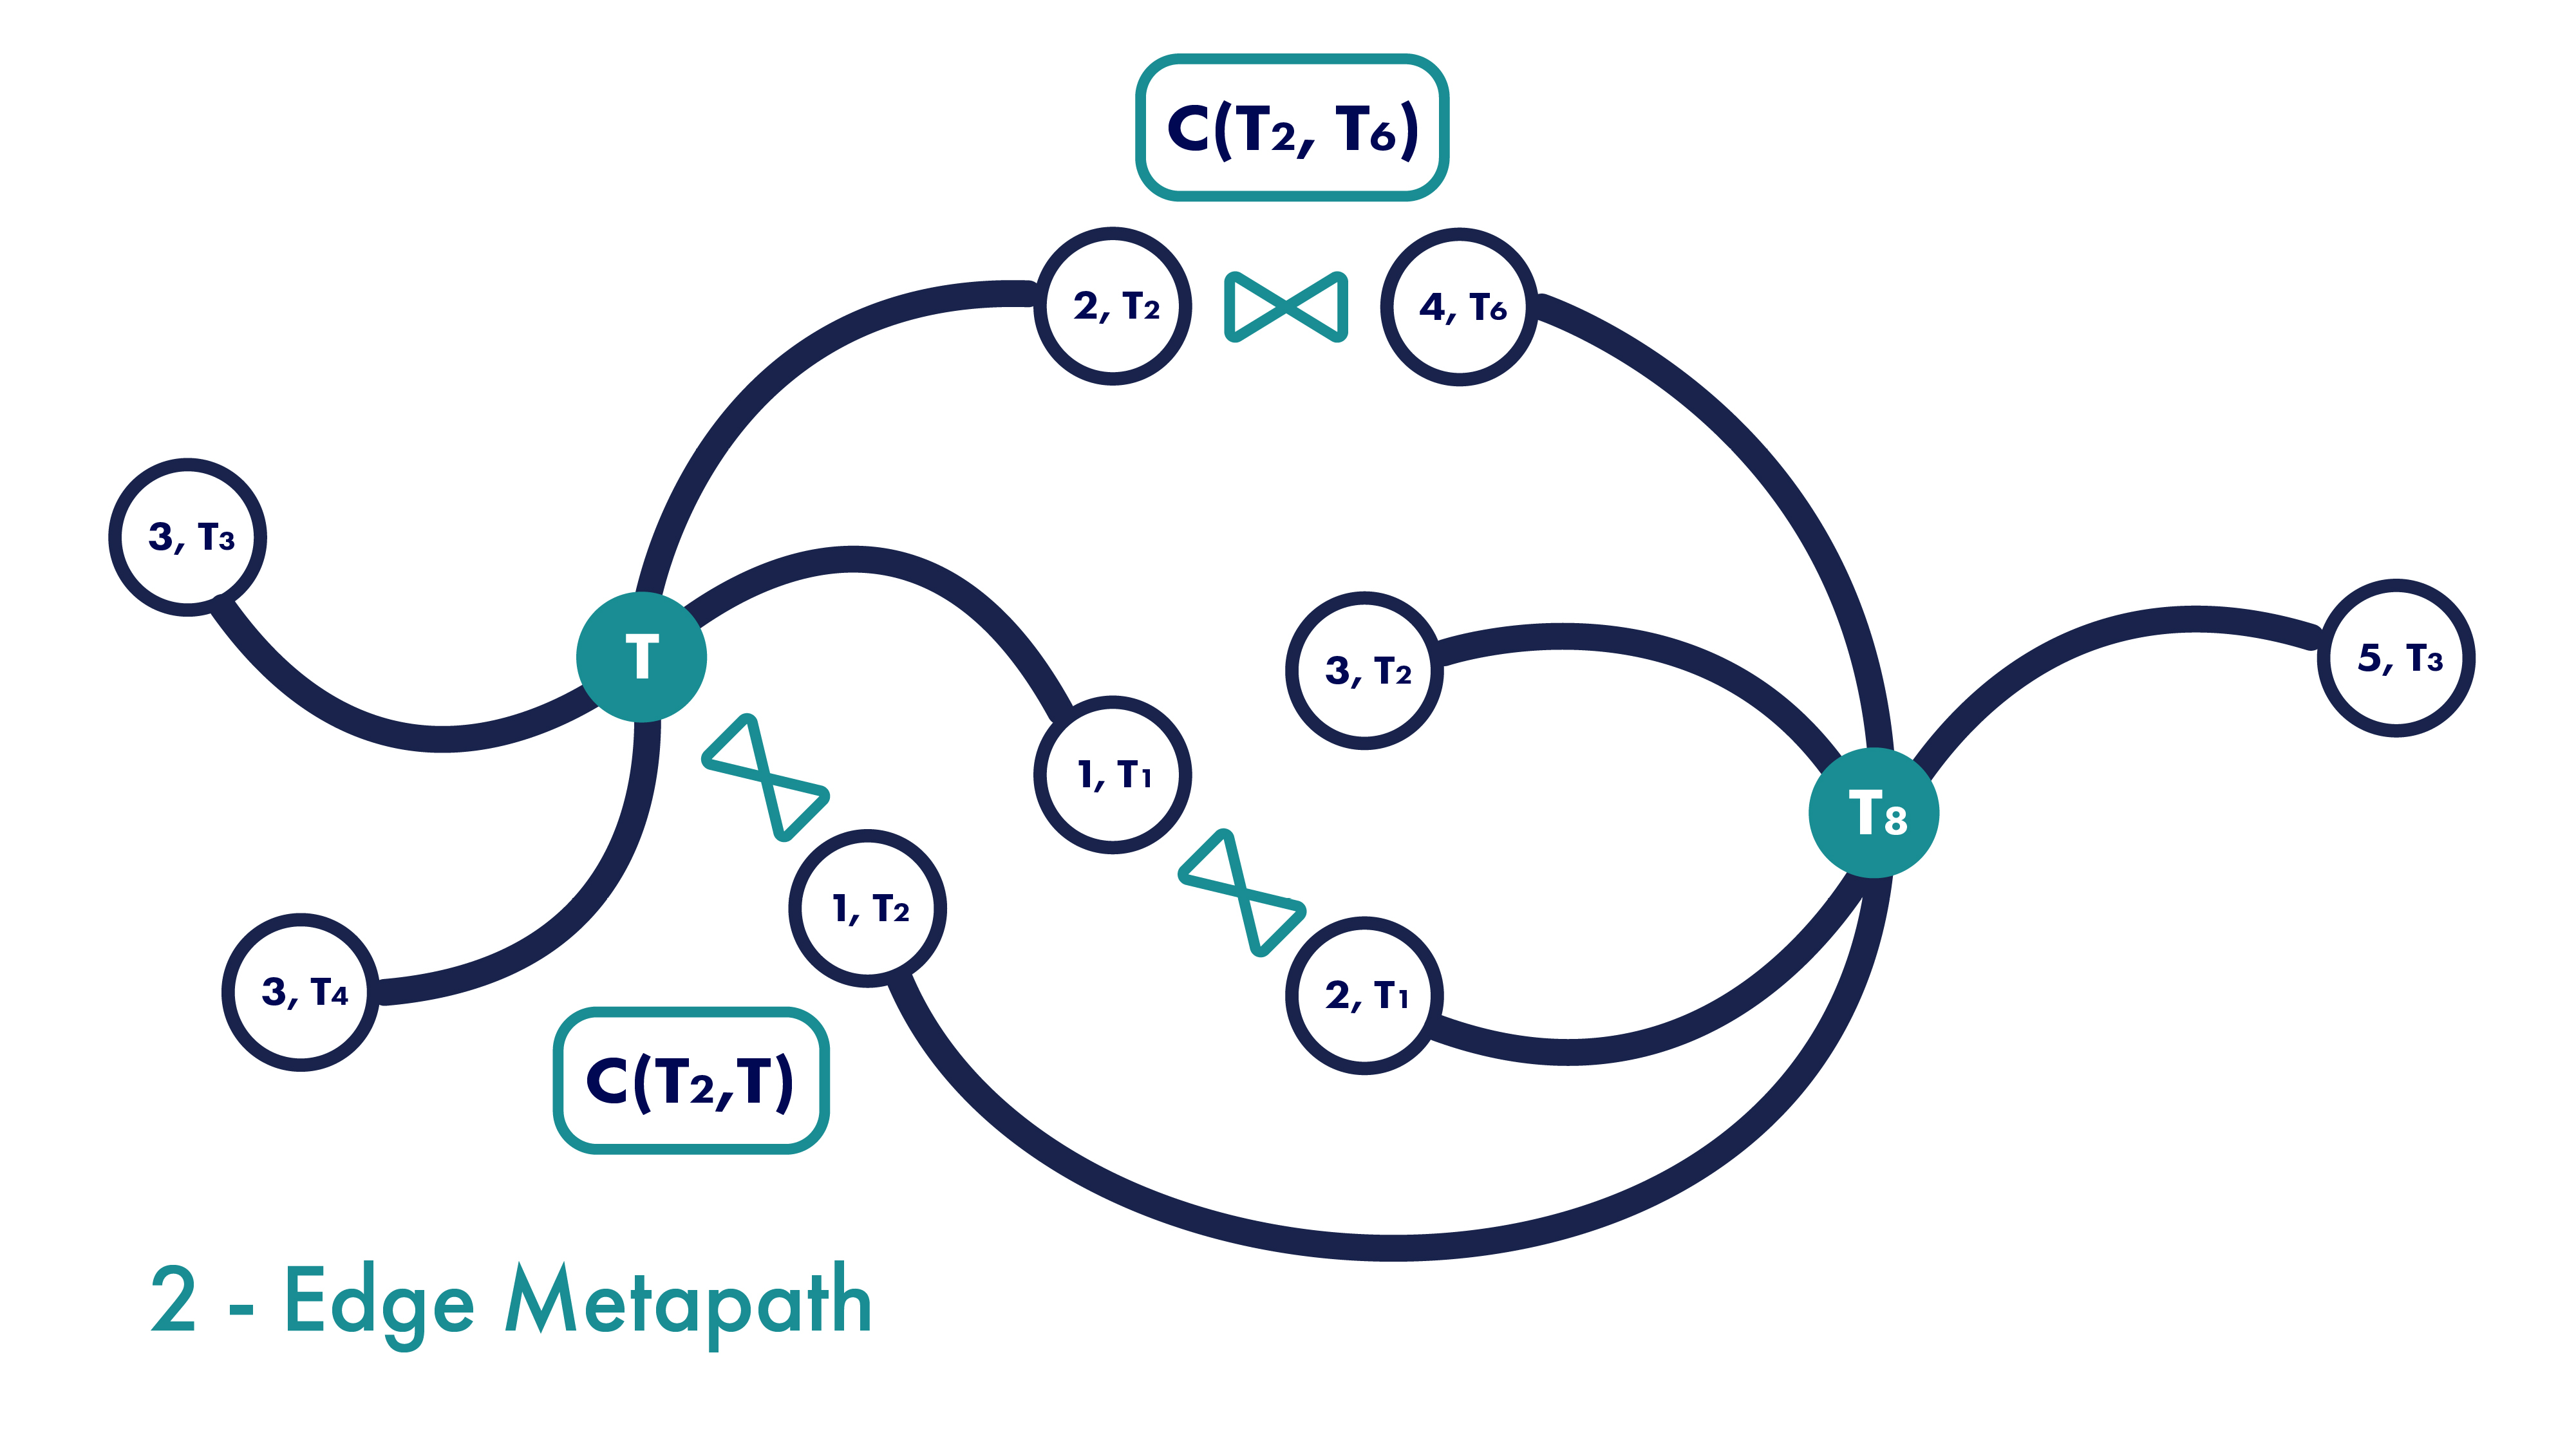
\includegraphics[width=0.65
\textwidth]{figures/Magistrale/typed_metapath}
\caption[Metapath]{A short metapath, formed by connecting two directed edges.
\label{fig:typed_metapath}}
\end{figure}

\subsubsection{Atoms}\label{sec:atoms}

The vertices (nodes) and edges (links) of a graph (metagraph), known as Atoms, are used to represent not only \enquote{data}, but also \enquote{procedures} and then, many metagraphs are executable programs as well as data structures. \\
Atoms are one of the main components of the AtomSpace. Atoms, together with Values are what the AtomSpace stores.  \\
The two primary types of Atoms are Nodes and Links. They are used to represent anything that resembles a graph-theoretical graph. \\
From the TMG definition above, Atoms are typed (in the sense of Type Theory) and thus, they can be used to store a large variety of information. 
Values are used to assign \enquote{valuations} to Atoms, to indicate the truth or likelihood of that Atom, or to hold other kinds of transient data. Every Atom has a key-value database attached to it, that can store any kind of information about that Atom. The distinction between the \enquote{shape of the graph}, and its related \enquote{data} is central for allowing high-speed graph traversal and generalized graph query. Note that, the name \enquote{Atom} was chosen because of the resemblance of OpenCog Atoms to the concept of atoms in mathematical logic. Moreover, in Ruby and Prolog programming languages, symbols are literally called atoms; in both LISP and Guile, allow parameters to be attached to symbols, as Values can be attached to Atoms. \\

When an atom are placed in the AtomSpace, it becomes unique: it gets a single, unique ID. Thus, in comparison to other programming languages\footnotemark{}, Atoms can be understood to be the same thing as symbols. The AtomSpace is essentially a symbol table, which commonly has the unique-symbols property. \footnotetext{Section \ref{sec:atomese} explains why it is possible to talk about programming languages}\\
The atom ID is the string name of a Node and the outgoing set of a Link. Specifically: Nodes are identified by their names or labels, that is the only property that they have. Links are identified by their contents, which are ordered or unordered sets of other atoms. Links do not have any name or label other than their contents: a link is uniquely identified by it's type and it's contents.\\
A TruthValue (a certain type of Values) gives each Atom a valuation or an interpretation and conseguently, all Atoms in a given, fixed AtomSpace always carry a default valuation/interpretation (i.e. a SimpleTruthValue) along with them. Naturally, an Atom may have one or more different kinds of TruthValues. \\
All TruthValues (tv) expose at least two parameters, representative of the SimpleTruthValue (stv):

\begin{enumerate}
	\item Strength: it represents a probability estimate of the true unknown probability. It is a floating-point value ranging from 0 to 1, with 0 denoting the classical Boolean false, and 1.0 denoting true.
	\item Confidence: it captures the spread of the second order distribution over the true unknown probability. It is a floating point value ranging from 0 to 1, expressing the certainty of the strength, with 0 denoting completely uncertain, and 1 denoting completely confident.
\end{enumerate}

The types form a type hierarchy: all atoms inherit from the type \enquote{Atom}, and the type Atom itself inherits from ProtoAtom. The ProtoAtom is itself the base type for Values as well as Atoms.
The atom type category site\footnotemark{} lists all documented theorized, proposed, currently in use, deprecated and obsolete atoms. \\
It is not a complete list: new types are easily invented, and the various OpenCog books mention Atom types that are not implemented or have been implemented in a different way. This reflects a more general point: the specific collection of Atom types in an OpenCog system is bound to change as the system is developed and experimented with. In the current system, it does not necessarily have a profound and lasting significance. \footnotetext{\url{https://wiki.opencog.org/w/Category:Atom_Types}}\\

Following a descriptive list of the main types of atoms used for this project:

\begin{itemize}
	\item \textbf{ConceptNode}: a Node representing any concept. \\
Its TruthValue, composed of at least a strength and a confidence value, has the strength that indicates the occurence of a concept within the context of experience and the confidence that indicates how sure the agent or system is of this value. 
\\
For example, imagine an empty AtomSpace and a newborn agent that begins observing the world for the first time. If the first two things it sees are a man and a cat, it may define the following concepts:

\begin{footnotesize}\textbf{Code in Scheme Programming Language notation:} \\
ConceptNode example.\end{footnotesize}
\begin{python}
	ConceptNode "man" (stv 0.5 0.001)
	ConceptNode "cat" (stv 0.5 0.001)
\end{python}

Since the agent has only observed two concepts in its universe, it will split in two the universe (and Strength accordingly): half (0.5) consists of men and the other half (0.5) consists of cats.
Because the agent has not made a lot of observations yet, it may assign a low Confidence to these values.

	\item \textbf{InheritanceLink}: a Link specify is-a relationships. \\
In the OpenCog system, basic InheritanceLinks are used to specify both intensional (is-a) and extensional (is-an-instance-of) relationships.

\begin{footnotesize}\textbf{Code in Scheme notation:} \\
InheritanceLink example, which specifies that a cat is an animal.
\end{footnotesize}
\begin{python}
	InheritanceLink
		ConceptNode "cat"
		ConceptNode "animal"
\end{python}

In this case, the TruthValue associated to InheritanceLink should be 0, if it is considered as extensional inheritance (inheritance between sets based on their members) and a value greater than 0 in the case of intensional inheritance (inheritance between entity-types based on their properties); obviously the value depends on how the agent assigns it.

	\item \textbf{PredicateNode}: it names the predicate of a relation. \\
Predicates are functions that have arguments, and produce a truth value as output. Predicates in OpenCog roughly resemble the predicate of first-order logic, but more general. It is very similar to a characteristic function in probability theory, which helps assign a floating-point truth value to a declaration. Its usege will be understood at later points. \\
Two interesting type of Atom that are derived from PredicateNode are \textbf{DefinedPredicateNode} and \textbf{GroundedPredicateNode}. \\
The first is a single atom that is attached to a more complex definition. During the evaluation of the predicate, its definition (typically some formula or other complex expression, constituted entirely of Atoms) is looked up and is used during evaluation. \\
The second specifies a predicate whose truth value is updated by the evaluation of a scheme, python or C++ code snippet. It is a \enquote{black box} from the point of view of logical inference and knowledge representation and it is used to interface to external data systems, for example, to robot motor control systems, or to sensory input systems. It is impossible to reason with it, as opposed to DefinedPredicateNodes, which are \enquote{clear boxes} whose inner workings are visible to inference, learning and analysis algorithms.

	\item \textbf{ListLink}: a Link used for grouping Atoms for some purpose, typically to specify a set of arguments to some function or relation. \\
The ListLink is best understood as a Cartesian product\footnotemark{}, because all of its uses involve passing an ordered sequence of arguments to some function or predicate. Ordered sequences can be naturally understood as Cartesian products, which is extremely general, cutting across all branches of mathematics.
\footnotetext{\url{https://github.com/opencog/atomspace/issues/1490\#issuecomment-352961503}}

	\item \textbf{EvaluationLink}: it provides a way for specifying the truth value of a predicate on a set of arguments. \\
The EvaluationLink is the most central and important atom type in OpenCog, as it is how OpenCog implements knowledge representation.

\begin{footnotesize}\textbf{Code in Scheme notation:} \\
EvaluationLink general structure, followed by a pratical example.
\end{footnotesize}
\begin{python}
	EvaluationLink <tv>
   		PredicateNode some_p
   		ListLink
       			SomeAtom val_1
       			OtherAtom val_2
\end{python}
This indicates that the predicate $some\_p$, applied to arguments $val\_1$ and $val\_2$, has the TruthValue $tv = some\_p(val\_1, val\_2)$. \\
Pratical example, $3 < 42$ is true:
\begin{python}
	 EvaluationLink <true_tv>
		PredicateNode "LessThan"
		ListLink
			NumberNode 3
			NumberNode 42
\end{python}

	\item \textbf{QueryLink}: it is used to specify a search pattern that can be grounded, solved or satisfied. Patterns consist of a set of clauses, with each clause containing one or more variables. When executed, the pattern matcher attempts to find groundings for the variables; that is, it attempts to find values for the variables such that the resulting graph exists in the AtomSpace. \\
QueryLink performs graph rewriting: after finding a match for a pattern, it uses the results to create a new pattern. \\
The QueryLink is a 2-ary or a 3-ary link, containing an optional variable declaration, followed by a pattern, followed by an implicand (consequent). In this project is used in a 3-ary form and thus, only the explicitly-declared variables are bounded. \\
QueryLink is treated as a graph re-write rule by the pattern matcher. That is, if the graph P (the antecedent) is found, then the graph Q (the consequent or implicand) is instantiated in the AtomSpace. If the graph Q is an \textbf{ExecutionOutputLink} atom type, such as in this project, then the specified Scheme/Python/C++/etc. routine is executed, with the rest of the ExecutionOutputLink contents passed as arguments. Conceptually, the pattern matcher acts to apply rules, specified as QueryLinks, to the contents of the AtomSpace. It implements a single step of a forward chainer.

\begin{footnotesize}\textbf{Code in Scheme notation:} \\
EvaluationLink general structure, followed by a pratical example.
\end{footnotesize}
\begin{python}
	QueryLink
		$variable_declarations	# optional
		P
		ExecutionOutputLink  	# graph Q
			GroundedSchemaNode "some-routine"
			ListLink
				A_1
				A_2
				...
\end{python}

The expression or predicate P is the pattern to be matched. The variables appearing in P are listed in the \$variable\_declarations. If a match to P is found, the variables are grounded with their matching atoms. The various A\_1, A\_2, etc. are created for each match, and are then passed as the first, second, ... arguments to a function \enquote{some-routine}. This function can then perform any action, for example drives external systems, such as motor controls or other devices.
\end{itemize}

There are other atom types used here. A more general list of Opencog atom types, which can be divided into categories, is the following:

\begin{itemize}
\item Arithmetic Atom Types: EqualLink, GreaterThanLink, NumberNode, IntervalLink, etc.
\item Boolean Atom Types: AndLink, OrLink, NotLink, etc. 
\item All atom types used for Natural Language Processing (NLP)
\item Atom types for the OpenCog Probabilist Logic Network
\item Atom types to perform Pattern Matching (PresentLink, AbsentLink, VariableList / VariableSet / VariableNode, etc.) 
\item Atom types for the threading 
\item Set-theoretical Atom Types: types having some form of set-theoretical signficance (MemberLink, SetLink, SubsetLink, etc.)
\item Atom types to perform searches over the AtomSpace (JoinLink, QueryLink, MeetLink, etc.) 
\end{itemize}

There is a type system for working with atom types: that is, the type of an atom can itself be specified using other atoms, which also applies to the polymorphic types. The type system allows for basic error checking, such as with the type checker, and more generally, it allows type-logical reasoning and inference to be performed on atom signatures. \\

In conclusion, the AtomSpace Explorer web tool can be used to display OpenCog data on screen. Atomese is fetched from the AtomSpace, then displayed as a two dimensional graph in the browser, Figure \ref{fig:atomspace_explorer} provides an example. \\

As closing note of this section, to greatly simplify the work in this project, uncertainty-free inference is used, so all TruthValues associated with atoms are always TRUE, that is what the robot \enquote{sees, does and thinks} has no probability of \enquote{failure}. But, as amply demonstrated above, the system is set up to work in completely uncertain environments and with uncertain reasoning. \\
Indeed, one of the most interesting modules of OpenCog is Probabilistic Logic Networks (PLN), a conceptual, mathematical and computational approach to uncertain inference. Although this project does not use it, it is particularly suitable for uncertain reasoning, especially when knowledge is based on limited observations of reality, but it can also handle abstract mathematical reasoning, and the relationship between the two, therefore this project could be integrated into it in the future. \\
PLN is currently used as a basic module for reasoning algorithms \cite{goertzel2008probabilistic, Goertzel2011RealWorldRT}. 

\begin{figure}[h]
\centering
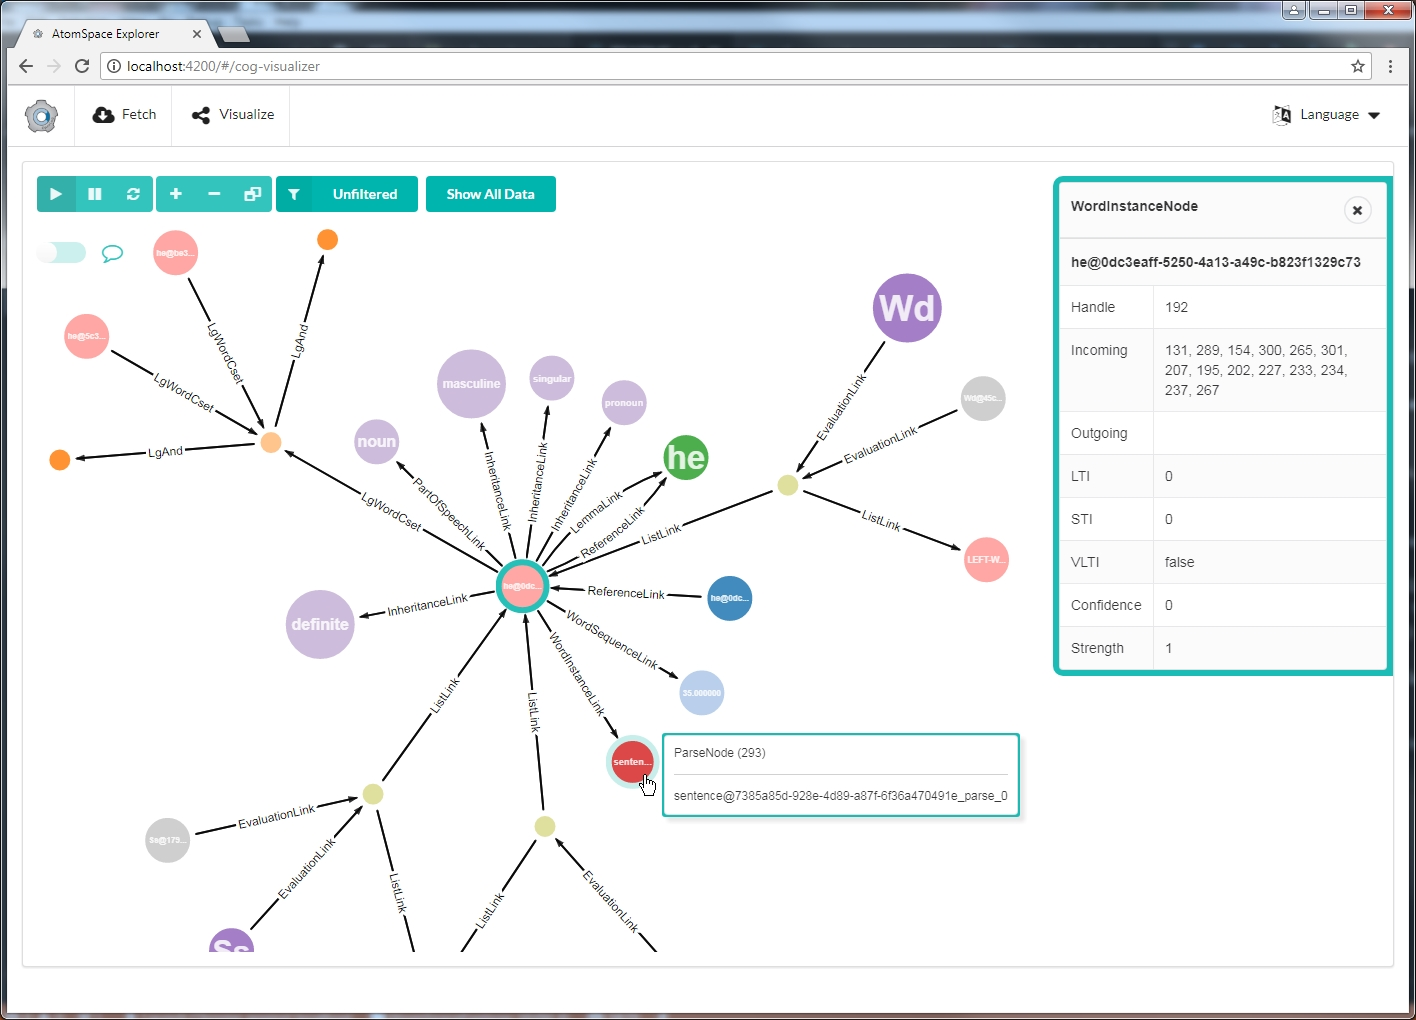
\includegraphics[width=1.0
\textwidth]{figures/Magistrale/atomspace_explorer}
\caption[AtomSpace Explorer ]{Atomspace example. By selecting an atom, you can get its unique ID, the type of atom (associated with an integer), incoming-set and outgoing-set, Strength and Confidence and much more.
\label{fig:atomspace_explorer}}
\end{figure}


\subsection{Atomese}\label{sec:atomese}

Because of these many and varied Atom types, constructing graphs to represent knowledge looks like a kind of \enquote{programming}. \\
The programming language is informally named \enquote{Atomese}. \\ 
Atomese is the concept of writing programs with Atoms. 
It vaguely resembles a strange mash-up of SQL, due to queriability, Prolog/Datalog, due to the logic and reasoning components, Lisp/Scheme, due to lambda expressions, Haskell/CaML, due to the type system, and rule engines, due to the graph rewriting and forward/backward chaining inference systems. \\

Atomese is not, and was never intended to be, a programming language with which humans would write source code, like Java, Python, LISP or Haskell. 
Rather, it is a language that computer algorithms, such as genetic programming systems, term rewriting systems and rule engines, would be able to manipulate. 
It is a graph database that pattern mining algorithms could search, manipulate and transform and is designed for easy self-introspection. \\

In its current form, Atomese was primarily designed to allow the generalized manipulation of large networks of probabilistic data by means of rules and inferences and reasoning systems. It extends the idea of probabilistic logic networks to a generalized system for algorithmically manipulating and managing data. The current, actual Atomese design has been heavily influenced by practical experience with natural-language processing, question answering, inferencing and the specific needs of robot control. \\

The use of the AtomSpace, and the operation and utility of Atomese, remains a topic of ongoing research (a re-evaluation of the OpenCog architecture is currently underway. A new OpenCog system called \enquote{Hyperon} is being studied \cite{goertzel_potapov_senna_singularitynet-opencog_team_2020}, introducing upgrades from Atomese to Atomese 2.0 \cite{DBLP:journals/corr/abs-2004-05267}, Distributed AtomSpace architecture \cite{distributed_2017, senna_2018, potapov_2020_1, potapov_2020_2} and much more) and design experimentation, as various AI and knowledge-processing subsystems are developed. These include machine learning, natural language processing, motion control and animation, deep-learning networks and vision processing, constraint solving and planning, pattern mining and data mining, question answering and common-sense systems, and emotional and behavioral psychological systems. Each of these impose sharply conflicting requirements on the AtomSpace architecture. The AtomSpace and Atomese are the current best-effort KR system for satisfying all these various needs in an integrated way.

\subsection{Pattern Engine, Unified Rule Engine and Relex2Logic}\label{sec:pattern_ur_engine}

Three more components of the OpenCog architecture are now introduced: Pattern Matcher, Unified Rule Engine and Relex2Logic. \\
Each of them is necessary for the following ones, in order of listing.
Unified Rule Engine is mostly built on top of the Pattern Matcher and it is applicable to rules written in a Scheme/Atomese representation, such as for Relex2Logic and PLN.

\subsubsection{Pattern Matcher}\label{sec:pattern_matcher}

OpenCog has a Pattern Matcher (PM), or Query Engine or Variable Unifier, that can be used to search the AtomSpace for specific patterns or arrangements or `templates' of atoms. 
The PM can be used from C++, Scheme or Python. \\
After specifying some (arbitrarily complex) arrangement of atoms, that is, a hypergraph consisting of Nodes and Links of several types, the PM can find all instances of that hypergraph in the AtomSpace. The pattern or template can have \enquote{holes} in it, locations that are variable, and so the pattern matcher can act to \enquote{fill in the blanks} when presented with a pattern that has blanks in it (better known by the expression: `grounding' a pattern). \\
For example, the VariableNode type are used to indicate these \enquote{blank spots}. \\
For a good introduction to these concepts, see \cite{baader_nipkow_1998}. Although, the PM implementation is considerably more sophisticated: it unifies multiple terms at once, automatically handles unordered terms (terms that can be in any order) and provides support for quotation, execution and evaluation. \\

For this project, patterns are specified using QueryLink type. \\
One creates the pattern-template that one wishes to search for. The pattern can be specified as a collection of trees, containing the VariableNodes, making up the graph. 
During the search, all matching graphs are found and the groundings are noted. \\
The QueryLink is used for graph-rewriting, thus these grounding are then pasted into a second pattern, to create a new graph. \\
In Section \ref{sec:domain_atomese}, practical applications will be presented to help understand these concepts as well.

\subsubsection{Unified Rule Engine}\label{sec:ure}

The Unified Rule Engine (URE) is a generic OpenCog rule engine operating on the AtomSpace and it can be used to implement any logic. \\
Two chaining modes are currently supported, Forward Chaining and Backward Chaining. \\
The strengths of the URE are:
\begin{itemize}
	\item Reads/writes knowledge directly from/to the AtomSpace
	\item It is generic, can be used to implement any logic, even higher order logics with some limitations
	\item Comes with a powerful control mechanism to speed up reasoning
\end{itemize}

It was used as a first approach to solve the problem faced in this project. It was later abandoned due to conceptual and practical problems in favour of a new approach, although, in the end, good ideas emerged that solved these problems. See related Section [...sviluppi futuri]. \\
For these reasons, any other information related to URE is referred to \cite{geisweiller_2019} and the webpages linked to that.
%% TODO
\subsubsection{Relex2Logic}\label{sec:r2l}

This project handles a Natural Language Processing (NLP) module. Here, some components of OpenCog this module superficially uses, are very briefly presented. \\
The component on the top is called Relex2Logic (R2L). \\
R2L produces a certain form of predicate-argument structure for an English-language sentence. That structure roughly resembles classical propositional or predicate logic, thus the name. \\
It is pointless to go into the details of this module because, first of all, it became obsolete because its java rule engine and representation scheme were inadequate and knowledge extraction was too far removed from the reasoning and anaphora components; secondly, because the predicate-argument structure is produced by applying a set of rules to the RelEx format (see below), using the forward chainer provided by URE, which require a very good knowledge of the topic in order to be understood. \\

Thus, this module takes as input an English sentence and returns a relatively simple logical representation of it in Atomese. That is, a hypergraph composed of atoms that are associated with the words of the sentence and then structured to express the logic of it in the form of a hypergraph. The following example is used to better explain: \\
\begin{python}
	The English sentence: "The cat is an animal"

---------------- Result:
(EvaluationLink (stv 1 1)
  (PredicateNode 
    "is.v@5fdee4a0-7ad4-4aa7-9172-55a137c3dbdf" 
      (stv 9.75697e-13 0.00124844))
  (ListLink
    (ConceptNode 
      "cat.n@e425545c-ceea-4eee-931b-a6c312d66d58")
    (ConceptNode 
      "animal.n@1813a95c-0c44-46f6-bad3-7232f6ff8616")))

(InheritanceLink (stv 1 1)
  (ConceptNode 
    "cat.n@e425545c-ceea-4eee-931b-a6c312d66d58")
  (ConceptNode 
    "animal.n@1813a95c-0c44-46f6-bad3-7232f6ff8616"))

(EvaluationLink (stv 1 1)
  (PredicateNode 
    "is.v@5fdee4a0-7ad4-4aa7-9172-55a137c3dbdf" 
      (stv 9.75697e-13 0.00124844))
  (ListLink
    (ConceptNode 
      "cat.n@e425545c-ceea-4eee-931b-a6c312d66d58")))

(InheritanceLink (stv 1 1)
  (InterpretationNode 
    "sentence@c9bf0479-2636-4a8b-901c-38d1305ed29e_
parse_0_interpretation_$X" (stv 9.75697e-13 0.00124844))
  (DefinedLinguisticConceptNode 
    "DeclarativeSpeechAct" (stv 9.75697e-13 0.00124844)))

(ImplicationLink (stv 1 1)
  (PredicateNode 
    "is.v@5fdee4a0-7ad4-4aa7-9172-55a137c3dbdf" 
      (stv 9.75697e-13 0.00124844))
  (PredicateNode "be" (stv 9.75697e-13 0.00124844)))

(InheritanceLink (stv 1 1)
  (ConceptNode "animal.n@1813a95c-0c44-46f6-bad3-7232f6ff8616")
  (ConceptNode "animal"))

(InheritanceLink (stv 1 1)
  (ConceptNode "cat.n@e425545c-ceea-4eee-931b-a6c312d66d58")
  (ConceptNode "cat"))

(InheritanceLink (stv 1 1)
  (PredicateNode 
    "is.v@5fdee4a0-7ad4-4aa7-9172-55a137c3dbdf" 
      (stv 9.75697e-13 0.00124844))
  (DefinedLinguisticConceptNode 
    "present" (stv 9.75697e-13 0.00124844)))

(EvaluationLink (stv 1 1)
  (DefinedLinguisticPredicateNode 
    "definite" (stv 9.75697e-13 0.00124844))
  (ListLink
    (ConceptNode 
      "cat.n@e425545c-ceea-4eee-931b-a6c312d66d58")))
\end{python}

All the Atoms whose names contain the \textit{@} character are those that are associated with the words in the sentence. In this way, the same word in different places can take on different meanings and links. \\
However, these atoms (such as \textit{cat.n@...}, \textit{animal.n@...} and \textit{is.v@...}) are actually inherited by the concepts (ConceptNodes) that represent them, so `cat', `animal' and `is' (lines 35, 41, 45). \\ 
Moreover, the atom in line 4 perfectly describes the relationship between these three concepts in the sentence. \\

The processing pipeline for a sentence is: 
\begin{enumerate}
	\item Sentence $\Rightarrow$ Link-Grammar
	\item Link-Grammar $\Rightarrow$ RelEx
	\item RelEx $\Rightarrow$ Relex2Logic
\end{enumerate}

Step 1 performs a syntactic parse of a sentence, using the Link Grammar (LG) parser. \\

Step 2 converts the LG output into a dependency grammar (DG) format that is more closely aligned with de-facto DG standards. This includes the unpacking of some of the LG output into standard linguistic feature classifications, e.g. for person, number, tense, aspect, mood, voice. \\
This converter is called RelEx, a Narrow-AI component of OpenCog. It is an English-language semantic dependency relationship extractor, built on the Carnegie-Mellon Link Grammar parser. It uses a series of graph rewriting rules to identify subject, object, indirect object and many other syntactic dependency relationships between words in a sentence. That is, it generates the dependency trees of a dependency grammar. \\
Unlike other dependency parsers, RelEx attempts a greater degree of semantic normalization: for questions, comparatives, entities, and for modifying clauses, and sub-ordinate clauses. \\

Step 3 extracts the predicate-argument logical structure, as shown above.

%!TEX root = ../dissertation.tex
\chapter{Problem Description} \label{cha:problem_description}

The problem addressed in this project is based on the classic blocks world problem\footnotemark{}. 
\footnotetext{\url{https://en.wikipedia.org/wiki/Blocks_world\#:~:text=In\%20its\%20basic\%20form\%2C\%20the,different\%20sizes\%2C\%20shapes\%20and\%20colors.}}
The blocks world is a planning domain in artificial intelligence and is used as a toy problem. From an algorithm perspective, it is an NP-Hard search and planning problem.
Here, a more general version of it is presented. \\
First of all, the environment consists of:
\begin{itemize}
	\item A robot manipulator, equipped with a video camera
	\item Blocks (cubes) in the same size, which all have an AprilTag \cite{olson2011tags, wang2016iros} attached to one of the faces
	\item Zero or more fixed objects, also with AprilTags
\end{itemize}

\begin{figure} [h]
\centering
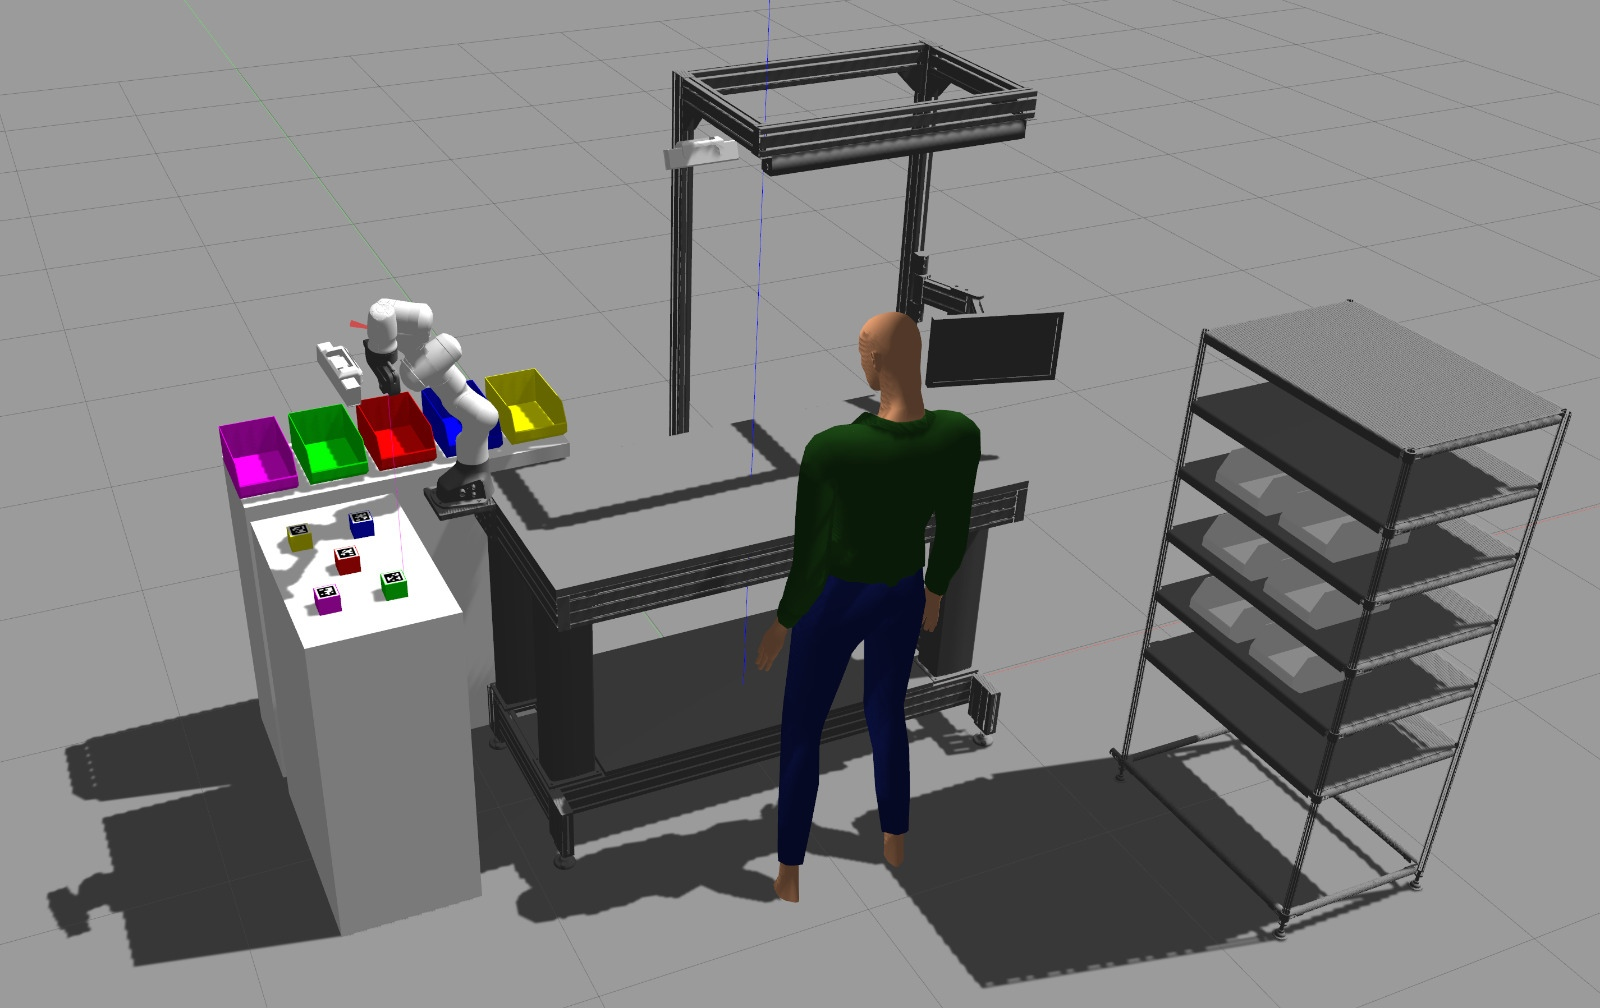
\includegraphics[width=0.9
\textwidth]{figures/Magistrale/env_1_temp}
\caption[Environment Configuration]{ IMMAGINE DA SISTEMARE
\label{fig:env_1}}
\end{figure} 

Figure \ref{fig:env_1} illustrates a possible configuration of the environment, which is the one used in this project. \\
Compared to the state-of-the-art, where the robot arm has to pick and place the blocks and the goal is to build one or more vertical stacks of them, the goal is generalized in a way that any arrangement of the blocks can be achieved. 
That is, given any initial arrangement of the blocks in the environment, find the shortest sequence of actions that the robot has to perform in order to achieve the required arrangement. \\

In order to define the implementation, it is first necessary to explain the constraints of this problem:

\begin{itemize}
	\item The robot knows only four actions: \textit{Pickup}, \textit{Putdown}, \textit{Stack}, \textit{Unstack}.
	\item Each block is \textit{clear} if and only if it has no object on it and is not \textit{in-hand} (i.e., the robot's hand can take it with a single action).
	\item Each block can be \textit{on} the table, on top of another object or \textit{in-hand}
	\item The robot's hand may be busy (it is holding a block) or free (it holds nothing)
	\item Only one block can be picked up at a time, putting it down before the next. It is not possible to pick up a block that is under another one (because it is not considered \textit{clear}) or to move a fixed object.
%% Aggiungi o rimuovi
\end{itemize}

The \textit{Pickup} action is the opposite of \textit{Putdown} and they are used to take/place a block from/on a fixed object. The \textit{Stack} action is the opposite of \textit{Unstack} and they are used to put/take a block on/from another block or a fixed object. \\
Basically these actions mirror physics. \\
For example, consider two blocks (A and B) on a table and block A is \textit{on} block B: to pick up block B, that block must be \textit{clear} and the hand must be free. Initially, block A is \textit{clear}, while B is not. Thus, one can do \textit{Unstack} of blocks A and B, getting block B \textit{clear} and block A \textit{in-hand}, then do \textit{Putdown} of block A and finally do \textit{Pickup} of block B, achieving the goal. Figure \ref{fig:blocks_example} illustrates these steps. \\

\begin{figure} [h]
\centering
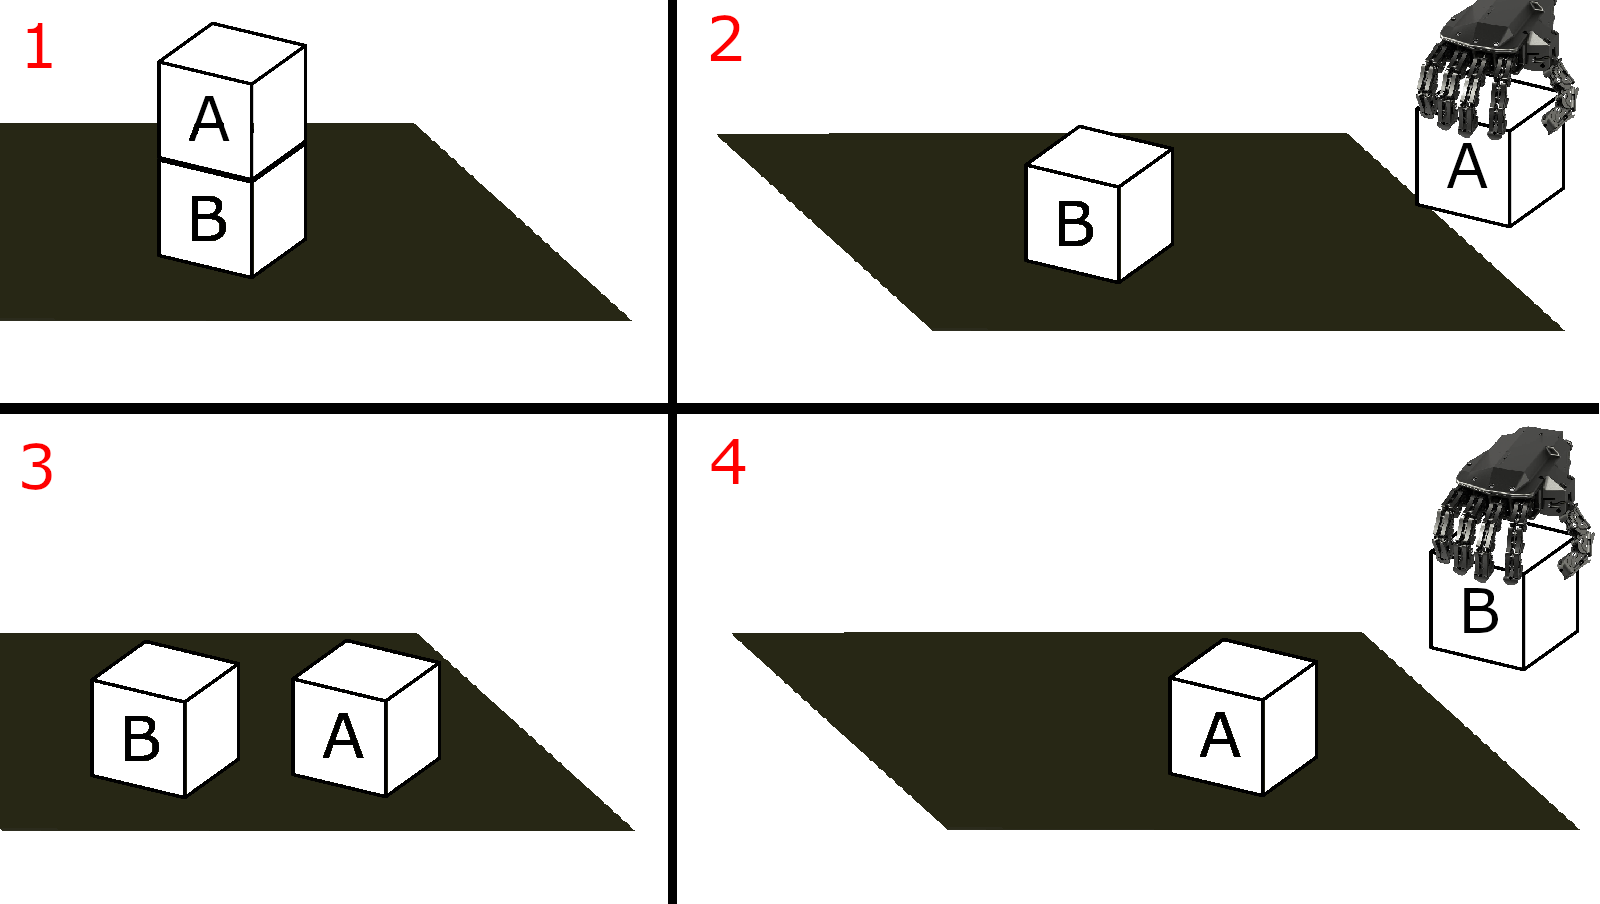
\includegraphics[width=0.9
\textwidth]{figures/Magistrale/blocks_example}
\caption[Blocks world example]{Three actions to go from state 1 (initial arrangement) to state 4 (target arrangement): \textit{Unstack} of A and B, \textit{Putdown} of A, \textit{Pickup} of B. 
\label{fig:blocks_example}}
\end{figure} 

Since it is possible to have more fixed objects (such as tables, shelves, etc.) than in the blocks world, where there is only a work plane, any free block can always be considered on top of something else. Consequently, the actions \textit{Pickup} and \textit{Putdown} lose their meaning because they become subcases of the respective \textit{Unstack} and \textit{Stack}. However, in this project all four are still maintained and used, as explained below. 


\section{Knowledge Base in Atomese}\label{sec:env_atomese}

Any aspect of the environment, the problem, the robot or anything else can be represented in the form of Atoms, which will populate the AtomSpace (i.e. the hypergraph of the KB). \\
There are many different ways of encoding these aspects. The one used in this project is proposed below. \\

Firstly, the Atomese representation of the objects: \\
\begin{python}
	(InheritanceLink
		(ConceptNode "apple")
		(ConceptNode "object"))

	(InheritanceLink
		(ConceptNode "table")
		(ConceptNode "fixed-object"))
\end{python}
On a practical (physical) level, the objects will all be cubes, except for the fixed ones. At the conceptual level, a semantic meaning will be associated to the AprilTags of each cube. In this way, and thanks to the AprilTags, it is possible to simplify the perception and manipulation of objects by replacing each different object with a cube. \\
In other words, it will be possible to \enquote{simulate} working with any kind of object, and thus demonstrate the potential of the NLP aspect of this project, leaving out perception and manipulation, which do not concern it at the moment. \\
For this reason, the code above speaks of \textit{apple} and not \textit{cube\_1}. \\

In that code, the \textit{apple} has been defined as an \textit{object} and the \textit{table} as a \textit{fixed-object}. 
ConceptNodes were used to refer to \enquote{concepts} and InheritanceLinks to connect two ConceptNodes with an \enquote{inheritance} meaning. This way, when the robot searches for which objects it can move, it will limit the pattern matching only to Atoms that are objects (thus, only to the apple). \\
As each atom is unique, it is not necessary to first define objects (i.e., \textit{apple} and \textit{table}) and concepts (i.e., \textit{object} and \textit{fixed-object}) and then, link them. Within the same AtomSpace, once an Atom is defined, whether independently or within any hypergraph, it will remain unique and the creation of other hypergraphs containing that Atom will not create a new one, but rather it will be shared between the various hypergraphs, in a sense, connecting them. \\

In addition, by construction of pattern matching rules, it is necessary to explicitly define the \enquote{non-equality} between all the various pairs of objects. Therefore, for example, given three objects such as \textit{apple}, \textit{tray} and \textit{table}, there will be Atoms like these: \\
\begin{python}
	(NotLink (EqualLink 
		(ConceptNode "apple") (ConceptNode "tray")))

	(NotLink (EqualLink 
		(ConceptNode "apple") (ConceptNode "table")))

	(NotLink (EqualLink 
		(ConceptNode "tray") (ConceptNode "table")))
\end{python}
They correspond to all possible simple combinations (without repetition) that can be constructed from the set of all objects (fixed ones included) taken two at a time. \\

Finally, now that the objects have been constructed, inherited and differentiated, one or more states must be associated with them. The best way to represent the state of an object is via an EvaluationLink, which associates a PredicateNode with one or more objects (their relative Atoms). The possible states of an object are: \textit{clear}, \textit{in-hand}, \textit{on}. Thus, for example: \\
\begin{python}
	(EvaluationLink
		(PredicateNode "clear")
		(ConceptNode "tray"))
	
	(EvaluationLink
		(PredicateNode "in-hand")
		(ConceptNode "apple"))
	
	(EvaluationLink
		(PredicateNode "on")
		(ListLink
			(ConceptNode "tray")
			(ConceptNode "table")))
\end{python}

In Appendix A, Section \ref{sec:KB_examples}, a complete examples have been added for further details.
%%  ovviamente si possono aggiungere un sacco di stati, attributi, etc. in più

\section{Actions in Atomese}\label{sec:domain_atomese}
Once the Atoms relative to the objects have been defined, the robot's actions must also be defined as hypergraphs. 
From this point on in the paper, these actions will also be called \enquote{rules}, being called rules the ones that are executed within AtomSpace for pattern matching. \\
Before exposing them, Section \ref{sec:PDDL} in Appendix A, provides the domain and problem in Planning Domain Definition Language (PDDL) notation of the standard block world problem.
Automated planning and scheduling problems are usually described in the PDDL notation, which is an AI planning language for symbolic manipulation tasks. \\
Starting from those definitions of the various actions, one can better understand how they are created in Atomese. 
Only the \textit{Pickup} rule is presented and explained here, as an example, whereas the code of the other three can be found in Appendix A, Section \ref{sec:action_atomese}. \bigskip \\
\begin{footnotesize}
\textbf{Code in Atomese notation:} \\
\textit{Pickup} action rule. 
\end{footnotesize}

\begin{python}
(define (pickup-action . args)
  (define precond (car (cdr args)))
  (define eff (car args))
  (cog-extract-recursive! precond)
  eff
)

(define (pickup args)
  (let 
    ((rule
      (if (equal? args `())
        (QueryLink
          (VariableList
            (TypedVariableLink 
              (VariableNode "?ob") 
              (TypeNode "ConceptNode"))
          ) ; parameters
          (AndLink
            (PresentLink
              (InheritanceLink
                (VariableNode "?ob")
                (ConceptNode "object"))
              (EvaluationLink
                (PredicateNode "clear")
                (VariableNode "?ob"))
            )
            (AbsentLink
              (EvaluationLink
                (PredicateNode "stacked")
                (VariableNode "?ob"))
            )
          )
          (ExecutionOutputLink
            (GroundedSchemaNode "scm: pickup-action")
            (ListLink
              ; effect
              (EvaluationLink
                (PredicateNode "in_hand")
                (VariableNode "?ob"))
              ; precondition
              (EvaluationLink
                (PredicateNode "clear")
                (VariableNode "?ob"))
            )
          )
        )
        (QueryLink
          (VariableList
            (TypedVariableLink 
              (VariableNode "?ob") 
              (TypeNode "ConceptNode"))
          ) ; parameters
          (AndLink
            (PresentLink
              (InheritanceLink
                (VariableNode "?ob")
                (ConceptNode "object"))
              (EvaluationLink
                (PredicateNode "clear")
                (VariableNode "?ob"))
            )
            (EqualLink
              (VariableNode "?ob")
              args
            )
            (AbsentLink
              (EvaluationLink
                (PredicateNode "stacked")
                (VariableNode "?ob"))
            )
          )
          (ExecutionOutputLink
            (GroundedSchemaNode "scm: pickup-action")
            (ListLink
              ; effect
              (EvaluationLink
                (PredicateNode "in_hand")
                (VariableNode "?ob"))
              ; precondition
              (EvaluationLink
                (PredicateNode "clear")
                (VariableNode "?ob"))
            )
          )
        )
      )
    ))
    rule
  )
)
\end{python}

The code is divided into two functions: \textit{(pickup-action . args)} and \textit{(pickup args)}. \\
The main rule (or action or function) is the second one, called \textit{pickup} (line 8), which describes the action of picking up some object.
It is composed of two large QueryLink atoms (lines 12 and 47), as for all other actions. \\
Only one of the two Atoms is used for each call of this function, via the conditional construct `if' (line 11). It checks whether the function has an argument \textit{args} other than empty \textit{'()}. 
If it is indeed empty, then the QueryLink from line 12 to 46 is used, otherwise the one from line 47 to 85, which actually uses the \textit{args} argument.
Indeed, initially the variable \textit{rule} is defined as one of the two QueryLinks, depending on the result of the conditional construct, and is then applied in line 88 (i.e., executing the QueryLink). \\
These QueryLinks are completely identical, except for the EqualLink atom on line 62.
Consequently, take a look first at the QueryLink with no argument, based on the generic description of a QueryLink in Section \ref{sec:atoms}.\\
It is composed of a parameter \textit{?ob} that is restricted to the ConceptNode type (lines 13-17). 
In this way, the rule will do pattern matching using the conditional part as a pattern, which will be parameterised by \textit{?ob} that will result as all possible objects that can be picked up, given the current composition of the AtomSpace. Thus, the notation "object (parameterized)" is given to generic objects that satisfy the requirements of parameterization. \\
The conditional part (or pattern) requires the logical and (AndLink) to be evaluated to TRUE (lines 18-32). This can only happen when both PresentLink and AbsentLink are evaluated to TRUE at the same time. 

\begin{itemize}
	\item AbsentLink is a trick to differentiate atoms simply \textit{clear} from those \textit{clear}, but also \textit{on} some other object; this corresponds to differentiating \textit{Pickup} and \textit{Unstack} actions (design choice). \\
Briefly, when an object is subjected to a \textit{Stack} action, a \enquote{stacked} state atom is created, and when it is subjected to \textit{Unstack}, that atom is removed from AtomSpace. \\
Finally, AbsentLink checks for the absence of that atom in AtomSpace: if the object (parameterized) is simply \textit{clear}, then the atom is not there and it can be picked up, otherwise the object (parameterized) is \textit{on} something else and the \textit{Unstack} action must be used instead of \textit{Pickup}. 
	\item PresentLink, the opposite of AbsentLink, verifies the presence in the AtomSpace of the atoms composing it, just like logical and, returns TRUE only when they are all found. \\
In this case, it verifies that the object (parameterized) is indeed an \textit{object} and that it is also \textit{clear}, from the definitions of the Pickup action.
\end{itemize}

The last part of the code (lines 33-45) is relative to the graph re-write and uses an ExecutionOutputLink atom to execute a GroundedSchemaNode. The GroundedSchemaNode behaves like the GroundedPredicateNode described in the previous section, but it is not associated with an EvaluationLink, it simply executes a Schema or Python code or Combo procedure. GroundedSchemaNode's preference, over GroundedPredicateNode, was a design choice to pursue the PDDL definition of the various actions. \\
In this project, it was decided to use a Schema code (line 34, `scm' stands for Schema) that executes the \textit{pickup-action} function, with a list of arguments provided by the ExecutionOutputLink. \\
This list of arguments (line 35) is made up of the effect and precondition of the Pickup rule. Therefore, the rule wants the object (parameterized) to be \textit{clear}, as a precondition, and the effect corresponds to the atom describing the state of the object \textit{in-hand}. \\
The \textit{pickup-action} function called (lines 1-6) takes these two atoms as arguments, removes from the AtomSpace the one corresponding to the precondition and finally, applies the effect, creating the relative atom in the AtomSpace. This is how the action takes place inside the AtomSpace: states that would no longer be "valid" after the action is executed are removed (such as the state of \textit{clear}, because the object (parameterized) will be in hand, thus no longer \textit{clear}) and those created due to the action are added (such as the state of \textit{in-hand}). \\

Now that the first QueryLink has been explained, the second behaves the same way, but with an additional constraint in the conditional part. \\
That constraint is the EqualLink in line 62 and it is used to limit the parameter (the VariabileNode) to coincide with the \textit{args} argument, which will be an atom corresponding to the object to be picked up, effectively restricting the pattern matching to that single atom. \\
In practice, the QueryLink with no argument performs the Pickup action on all objects that can actually be picked up, instead of the QueryLink with argument that do \textit{Pickup} only on the object passed as argument. That is, the first shows which objects are takeable, the second actually takes one. \\
The reason why these two possibilities (the two QueryLinks) are needed will be better understood when the algorithm will be discussed (Chapter [...]). 

 
%!TEX root = ../dissertation.tex

\chapter{System Implementation} \label{cha:algorithm}

Having defined the OpenCog system and part of the implementation of the problem in the previous chapters, it is now possible to combine all the various modules and explain the functioning of the internal design and the main algorithm. \\

It is possible to divide the entire project into 6 phases: initial, perception, learning, request, search and results execution.  

\section{Initial Phase}\label{sec:init}

The initial phase concerns the initialization of the simulated environment. The framework used for the development and programming of the robot is the well-known ROS, Melodic version, and the Gazebo 9 system handles the simulation. 
Therefore, the world as in Figure \ref{fig:env_2_named} is loaded into Gazebo. 
It consists of a robot manipulator with an attached camera, some fixed objects (such as tables, workbench and bins) and cubes, both with their AprilTags used for detection and semantic assignment. 
Then, a server in C++ code is activated and the nodes of the ROS system for robot control and object perception become available for listening. 
Finally, the main AtomSpace is created and the actions rules are loaded into it. 

\begin{figure} [h]
\centering
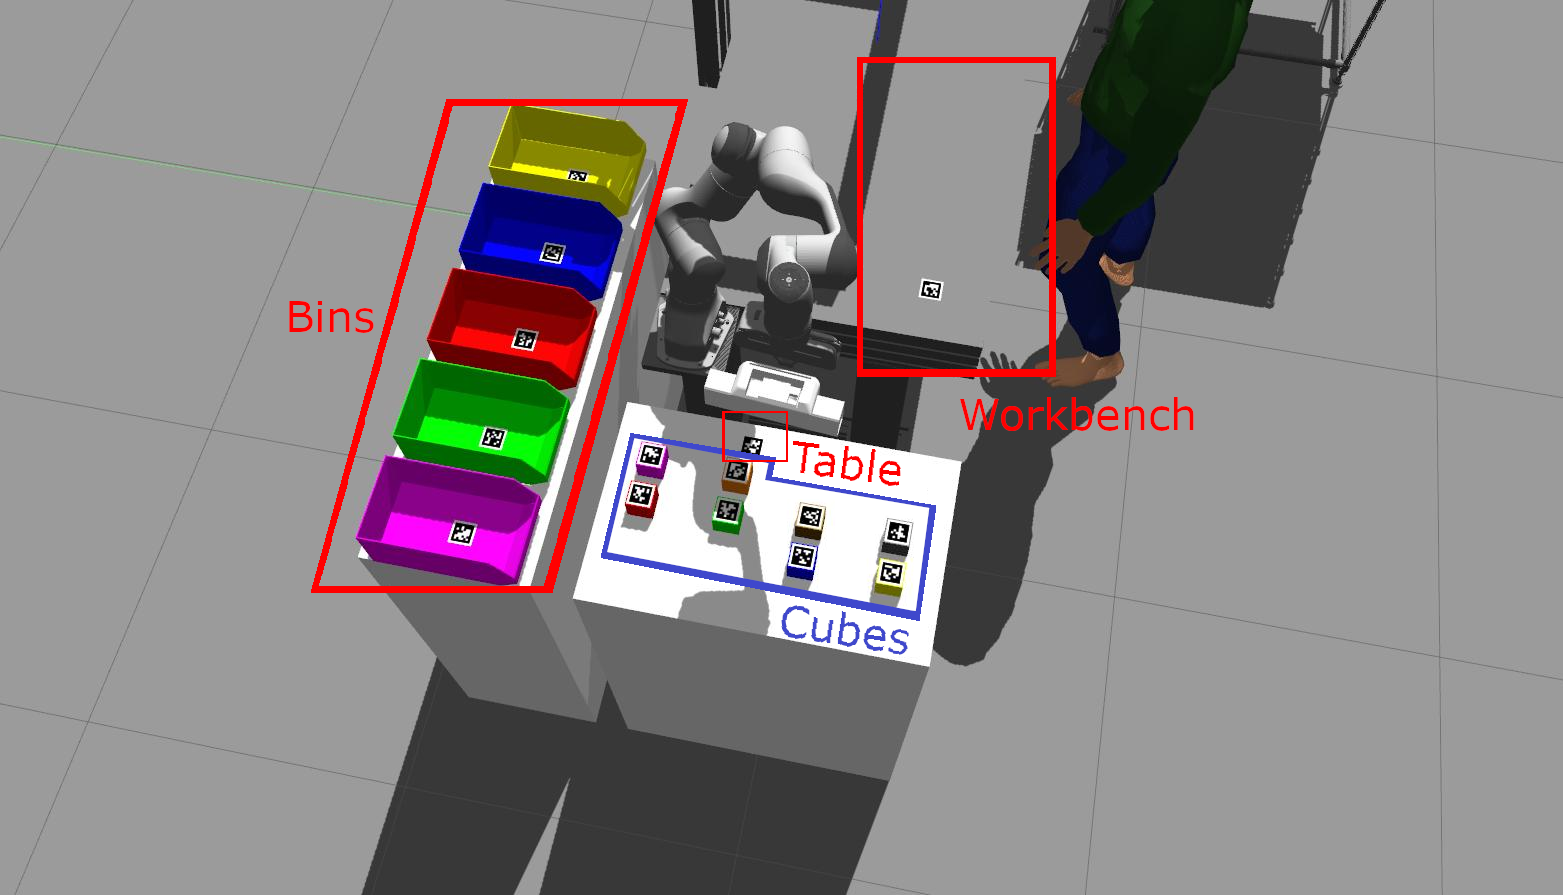
\includegraphics[width=1.0
\textwidth]{figures/Magistrale/env_objs}
\caption[Environment Components Description]{ In the red boxes are collected the objects that are considered fixed. Meanwhile, the blue box contains the remaining objects, represented by cubes.
\label{fig:env_2_named}}
\end{figure} 

\section{Perception Phase}\label{sec:perception}

The perception phase, like the remaining phases, is written in Python code and sends commands via a Python client to the C++ server mentioned above. These commands move the robot and allow it to scan its surrounding area for possible objects (related AprilTags are recognised), thanks to the camera attached to the top of it. \\
Of each AprilTag found, its associated semantic representation (i.e., English word describing the object, as well as the name of its relative ConceptNode, thus, for example: \enquote{table}, \enquote{workbench}, etc.) is returned by the server to the client, which in turn returns it to the main Python code that begins the initialization of the objects list, found in the environment.

\section{Learning Phase}\label{sec:learning}

The learning phase is used to provide additional information. 
The perception algorithm is extremely simple and does not deal with information processing. Consequently, it is not able to distinguish an object from a fixed object or to infer that an object is placed on top of another. Surely, with a perception processing module all of this, and much more, could be managed. 
However, this project shows the simplicity of integration and the potential of the learning with the OpenCog system. \\

This phase was created to tell the robot which objects are fixed, which are on top of others (fixed objects excluded) or which one is in the robot's hand. That is, to provide the necessary additional information, which the simple perception phase does not perceive, to describe the initial situation of the environment.
This is done by a module using NLP, consisting of the Relex2Logic OpenCog module and a post-processing phase. \\

Additional information is provided to the system via English sentences. 
This module applies Relex2Logic to these sentences, creating the hypergraph describing them within a new empty AtomSpace (process explained in Section \ref{sec:r2l}).  
Next, the post-processing phase loads the rules presented in Section \ref{sec:NLP} and executes them within that AtomSpace. Those rules look for patterns corresponding to the possible information that the system might need and create summary atoms that can be easily used by the algorithm. Thus, from the results obtained by Relex2Logic, they infer atoms such as the ones shown in Section \ref{sec:env_atomese}, which are then added to the main AtomSpace. \\

Moreover, from the information learned in this phase, the \textit{clear} state atoms of the effectively free objects and the \textit{object} inheritance atoms of the non-fixed objects are created.  
Finally, the last atoms of the initial KB are added to the main AtomSpace. They are all possible simple combinations (without repetition) from the objects list taken two at a time (explained in Section \ref{sec:r2l}, too). 
The main AtomSpace is now complete and fully describes the initial situation. 

\section{Request Phase}\label{sec:request}

The request phase behaves like the previous one, except for the aim. Whereas before, English sentences are used to give additional information, now new English sentences are requested to define the goal to be achieved. 
To define the goal it is not necessary to describe the final complete arrangement of objects in the environment, but just the states of the objects one wants to achieve. 
Thus, the same steps used in the learning phase are performed here. That is, the English sentences are processed to obtain the corresponding set of atoms that describes them. Then, these atoms are added to a goal list used by the algorithm to find a solution.

\section{Search Phase}\label{sec:search}

The search phase contains the actual implementation of the algorithm and corresponds to the core of the system. It tries to achieve an arrangement of objects in which all atoms in the goal list are satisfied.
To find a solution, the AtomSpace of the final arrangement must contain every atom within the goal list. \\

Since each atom is unique in the AtomSpace, two AtomSpaces describing the same arrangement and state of objects have the same atoms, thus they are identical. 
Consequently, each possible arrangement of objects in the environment can be associated with one and only one AtomSpace, making it a de facto state of a Finite State Machine (FSM).
Moreover, each of the four actions available to the robot can be seen as a step of this FSM. 
Starting from a certain state, performing an action leads that state (i.e., that AtomSpace) into a new one. However, from each state, one or more actions can be performed and thus, one or more states can be reached. \\

One of the best ways to handle this structure is through a tree that has AtomSpaces as tree-nodes (to distinguish them from Nodes in Atomese) and available actions as tree-edges.
In addition, each tree-node has a label describing the action used, and on which objects, by its parent to create it.
In this way, each branch of the tree describes a different sequence of actions. They can be derived by starting with a solution tree-node and reading the labels of the parent tree-nodes backwards until the root, adding each label to a list. Finally, reversing the list.  \\

After the request phase, the root of the tree, containing the main AtomSpace and a \textit{NULL} label, is created. 
Next, the search algorithm, based on the well-known Breadth-First Search (BFS) (more details in \cite{BFS-wiki, BFS}), expands the tree in search of a solution.

\subsection{BFS-Based Algorithm}\label{sec:bfs_search}

The BFS-based algorithm is recursive and accepts as arguments a tree-node and a variable, which limits the actions to be performed. 
Following the rules of the problem (Secion \ref{cha:problem_description}), it is trivial to deduce that the actions alternate for each step of the algorithm.
That is, starting from the root:

\begin{enumerate} 
	\item If there exists an atom, within the AtomSpace contained in the root, that describes the \textit{in-hand} state of an object, then only \textit{Stack} and \textit{Putdown} actions can create children. Conversely, if there are no objects in hand, only the actions of \textit{Pickup} and \textit{Unstack} can. This is because the current state of the robot's hand limits the action used to go to the next state. If the hand is free, it can only grab an object, while if it is busy, it can only place the object down.

	\item From this first intuition, follows the one applicable to each step: given a certain tree-node, if the action \textit{Stack} or \textit{Putdown} created it, then the children of that node can only be created by \textit{Pickup} or \textit{Unstack} actions, otherwise vice versa.
\end{enumerate}

This is the reason why the BFS-algorithm has a variable as the second argument, it holds the action used to create the node in the first argument. 
Trying all the actions at each step would also give the same result, but additional atoms would have to be added to the rule pattern to check whether the hand is free or busy.
Instead, following this design simplifies the rules, speeds up the algorithm and avoids unnecessary code execution.


\subsubsection{Termination Criteria of the BFS-Based Algorithm}\label{sec:term_criteria}

Some additional parameters are defined to limit and improve the search. As a result, it is possible to use 4 different searches:

\begin{enumerate}
	\item Search until a first solution is found.
	\item Search restricted to a maximum number of iterations.
	\item Explore the whole tree.
	\item Quick search.
\end{enumerate}

The quick search finds a solution, decreasing the number of iterations in most situations.
As this type of problems suffers from combinatorial explosion\footnotemark{}, the number of tree-nodes grows exponentially as the tree expands.
\footnotetext{\url{https://en.wikipedia.org/wiki/Combinatorial_explosion}} 
One way to reduce this expansion is to limit the available actions to only those that interact with one or more objects appearing in the goal list.
Many unnecessary actions are avoided, however this makes the algorithm incorrect, since the certainty of finding a solution is lost.
It still works well for most initial arrangements and goal lists and if it fails, the search in point 1 (which is correct if a solution exists, like searches in points 2 and 3) can be used. \\

Finally, a solution is found when all the atoms composing the goal list are within the AtomSpace of a tree-node. 
Furthermore, the first solution found will certainly be the optimal solution, i.e. the solution that uses the minimum number of actions to go from the initial arrangement of objects to the goal one.
This is because for each tree-node, before being expanded, its AtomSpace is compared with the one of any tree-node belonging to its same branch.
If a match is found (i.e., they are identical), then the algorithm has come back to an arrangement of objects it has already encountered and thus, the sequence of subsequent actions would be a repetition of that associated with the matched tree-node. Consequently, the expansion of this tree-node ends.


\subsubsection{Steps of the BFS-Based Algorithm}\label{sec:step_search}

From the definitions above, it is now possible to list the steps that the BFS-based algorithm goes through. 
The first recursive call has as arguments the root node (containing the main AtomSpace) and the variable defined according to the state of the hand.
Inside each call:

\begin{enumerate}
	\item It is checked if the maximum number of iterations is reached (in the case of limited search). As a consequence, the algorithm returns or continues.
	
	\item It is checked if the AtomSpace, contained in the tree-node argument, satisfies all the atoms in the goal list. If satisfied, this tree-node is added to the solution list and the algorithm returns or continues depending on the type of search.
	
	\item It is checked that the AtomSpace, contained in the tree-node argument, has not been encountered before. If encountered, this tree-node is not expanded and the algorithm moves on to the next one (Go back to point 1), otherwise its expansion begins.
	
	\item Now that the checks have been passed, the expansion of the tree-node argument occurs. 
According to the variable argument, only two of the four actions can be executed.
Thus, from the AtomSpace of the current tree-node, two AtomSpace children (two copies of the parent) are created, one for each action. \\
Then, for each action (rule), the respective QueryLink without argument (i.e., the one that returns all possible objects that match the pattern; i.e., the objects on which that action can be performed), is executed within the AtomSpace assigned to it. \\
It is necessary to use AtomSpace copies because rule execution adds and removes atoms within AtomSpace and thus, modifies it. This means that executing a QueryLink without arguments modifies the AtomSpace as if the related action had been executed on all the matched objects at the same time, leading the AtomSpace into an incorrect state. 
To summarise: 

	\begin{enumerate}
		\item AtomSpace copies are created
		\item Rules on generic objects are executed, one in each AtomSpace
		\item The objects, returned as solutions of the rules, correspond to the objects on which actions can be executed. They are stored in a list for each action.
		\item AtomSpace copies are cleaned up and deleted.
	\end{enumerate}

	\item Finally, for each object found, a copy of the AtomSpace of the tree-node argument is created again. Based on the list to which the object belongs, the corresponding action is executed in that AtomSpace, but this time using the QueryLink with the argument, which corresponds to that object. That is, the action is only executed on that object. 
The resulting AtomSpaces are associated with new tree-nodes and become the children of the tree-node argument.
	
	\item At last, these new tree-nodes, obtained by executing the two actions available to each object on which they are applicable, are then added to a FIFO queue.
This queue is used for BFS. 
The expansion of this tree-node is finished and the tree-node at the top of the queue is extracted and passed to a new recursive call of this algorithm, together with the variable describing the action used previously in its branch. 
\end{enumerate}


\section{Results Execution Phase}\label{sec:results_exec}

At the end of the search phase, the solution list contains the tree-nodes having an AtomSpace that satisfies all the atoms in the solution list.
As already explained in Section \ref{sec:search}, from each solution tree-node, a list containing a sequence of actions can be extracted.
If the solution list is not empty, then the first result corresponds to the optimal solution, otherwise either there is no solution or the search parameters need to be changed. \\
In conclusion, the optimal solution is sent from the client to the server, which will command the robot to perform each of those actions in sequence, thus achieving the required arrangement of objects.

\section{Practical Example}\label{sec:alg_example}

The following steps provide a simple practical example in order to clarify and contextualise the above phases.

\begin{enumerate}

	\item Initial Phase: \\
Loading environment (Ros, Gazebo, Relex2Logic Server, Cubes, AprilTags, etc.).

	\item Perception Phase: \\
Assume that four AprilTags are detected. Assume also that the AprilTags associate tree objects with a semantic meaning corresponding to parts of an industrial product to be assembled and the fourth with \enquote{workbench}. For simplicity in this example, the parts will be called \enquote{screw}, \enquote{bolt} and \enquote{washer}.

	\item Learning Phase: \\
The only additional information needed by the robot is: \enquote{The workbench is a fixed object.}. From this sentence the following atom will be extracted:
\begin{python}
	(InheritanceLink
		(ConceptNode "workbench")
		(ConceptNode "fixed-object"))
\end{python}

	\item Request Phase: \\
Assign an easy task: \enquote{The washer is on the screw. The bolt is on the washer.}.  From these sentences the following atoms will be extracted:
\begin{python}
	(EvaluationLink
		(PredicateNode "on")
		(ListLink
			(ConceptNode "washer")
			(ConceptNode "screw")))

	(EvaluationLink
		(PredicateNode "on")
		(ListLink
			(ConceptNode "bolt")
			(ConceptNode "washer")))
\end{python}

	\item Search Phase: \\
The Figure \ref{fig:BFS_1} shows the first steps of tree expansion using the BFS-based algorithm.
First, the hand is free, thus the algorithm will try to do \textit{Pickup} and \textit{Unstack} actions. Since \textit{screw}, \textit{bolt} and \textit{washer} are \textit{clear} objects, the first iteration of the algorithm will create 3 tree-nodes corresponding to the initial object arrangement (i.e., the arrangement of the root), except the one to which \textit{Pickup} is performed. \\
The \textit{workbench} is a fixed object, thus it is not found as a solution of \textit{Pickup}, moreover the action \textit{Unstack} returns an empty result because there are no stacked objects\footnotemark{}.
\footnotetext{The objects are actually stacked relative to the workbench. However, this fixed object can be considered as the initial one and therefore one can ignore the stacks and use actions of \textit{Pickup} and \textit{Putdown}, alternatively the stacks can be added as information during the learning phase and consequently, actions of \textit{Stack} and \textit{Unstack} will be used instead.}
\\Subsequently, these tree-nodes are analysed following the order corresponding to the blue numbers in the figure. None of them is a solution tree-node or has an AtomSpace already encountered, thus, their children are created. \\
Tree-node number 4 is obtained by making \textit{Pickup} of A and then \textit{Putdown} of the same, so its AtomSpace will correspond to the one of the root. Consequently, its expansion ends. \\
The expansions continue until the yellow tree-node is reached, which has an AtomSpace containing all the atoms in the goal list. Therefore, a solution is found and the search ends (Quick search).
The sequence of actions from the initial arrangement to the goal arrangement can easily be read from the tree-edges, going up the branch from the yellow tree-node to the root.

\begin{figure} [h]
\centering
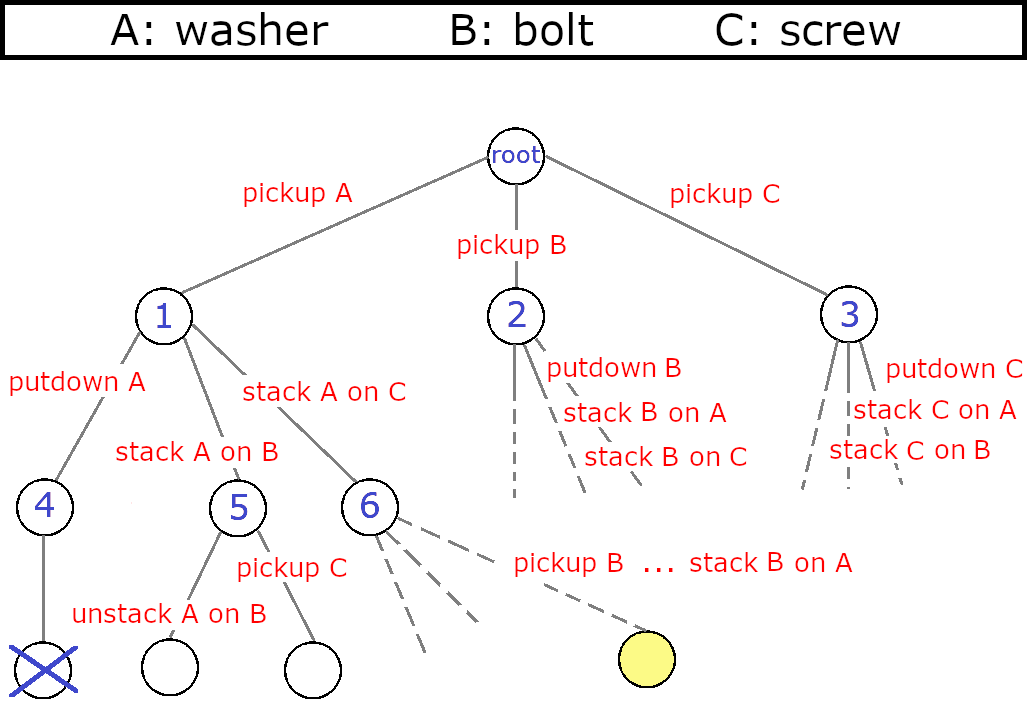
\includegraphics[width=1.0
\textwidth]{figures/Magistrale/BFS_1_blue}
\caption[BFS Example]{Graph describing the expansion of the tree of the practical example.  \\
Each node contains an AtomSpace and each edge describes an action. \\
Each AtomSpace at an internal node is unique among all those contained in its branch. With the exception of AtomSpaces at leaf nodes that either already exist within its own branch (node marked with a blue X) or are a solution (yellow node). \\
The order of node expansion is shown by the sequence of numbers within them and follows the order of the BFS. \\
The legend on the top simplifies the labels in the tree by using the letters A, B, C instead of names used in the algorithm. 
\label{fig:BFS_1}}
\end{figure} 

	\item Results Execution Phase: \\
The following sequence of actions will be performed by the robot, satisfying the initial request:
\begin{python}
	- Pickup washer
	- Stack washer on screw
	- Pickup bolt
	- Stack bolt on washer
\end{python}
\end{enumerate}
%!TEX root = ../dissertation.tex
\chapter{Conclusione}
\label{conclusione}

Lorem ipsum dolor sit amet, consectetuer adipiscing elit. Morbi commodo, ipsum sed pharetra gravida, orci magna rhoncus neque, id pulvinar odio lorem non turpis. Nullam sit amet enim. Suspendisse id velit vitae ligula volutpat condimentum. Aliquam erat volutpat. Sed quis velit. Nulla facilisi. Nulla libero. Vivamus pharetra posuere sapien. Nam consectetuer. Sed aliquam, nunc eget euismod ullamcorper, lectus nunc ullamcorper orci, fermentum bibendum enim nibh eget ipsum. Donec porttitor ligula eu dolor. Maecenas vitae nulla consequat libero cursus venenatis. Nam magna enim, accumsan eu, blandit sed, blandit a, eros.

Quisque facilisis erat a dui. Nam malesuada ornare dolor. Cras gravida, diam sit amet rhoncus ornare, erat elit consectetuer erat, id egestas pede nibh eget odio. Proin tincidunt, velit vel porta elementum, magna diam molestie sapien, non aliquet massa pede eu diam. Aliquam iaculis. Fusce et ipsum et nulla tristique facilisis. Donec eget sem sit amet ligula viverra gravida. Etiam vehicula urna vel turpis. Suspendisse sagittis ante a urna. Morbi a est quis orci consequat rutrum. Nullam egestas feugiat felis. Integer adipiscing semper ligula. Nunc molestie, nisl sit amet cursus convallis, sapien lectus pretium metus, vitae pretium enim wisi id lectus. Donec vestibulum. Etiam vel nibh. Nulla facilisi. Mauris pharetra. Donec augue. Fusce ultrices, neque id dignissim ultrices, tellus mauris dictum elit, vel lacinia enim metus eu nunc.

Pellentesque habitant morbi tristique senectus et netus et malesuada fames ac turpis egestas. Vestibulum tortor quam, feugiat vitae, ultricies eget, tempor sit amet, ante. Donec eu libero sit amet quam egestas semper. Aenean ultricies mi vitae est. Mauris placerat eleifend leo. Quisque sit amet est et sapien ullamcorper pharetra. Vestibulum erat wisi, condimentum sed, commodo vitae, ornare sit amet, wisi. Aenean fermentum, elit eget tincidunt condimentum, eros ipsum rutrum orci, sagittis tempus lacus enim ac dui. Donec non enim in turpis pulvinar facilisis. Ut felis.

Cras sed ante. Phasellus in massa. Curabitur dolor eros, gravida et, hendrerit ac, cursus non, massa. Aliquam lorem. In hac habitasse platea dictumst. Cras eu mauris. Quisque lacus. Donec ipsum. Nullam vitae sem at nunc pharetra ultricies. Vivamus elit eros, ullamcorper a, adipiscing sit amet, porttitor ut, nibh. Maecenas adipiscing mollis massa. Nunc ut dui eget nulla venenatis aliquet. Sed luctus posuere justo. Cras vehicula varius turpis. Vivamus eros metus, tristique sit amet, molestie dignissim, malesuada et, urna.

Cras dictum. Maecenas ut turpis. In vitae erat ac orci dignissim eleifend. Nunc quis justo. Sed vel ipsum in purus tincidunt pharetra. Sed pulvinar, felis id consectetuer malesuada, enim nisl mattis elit, a facilisis tortor nibh quis leo. Sed augue lacus, pretium vitae, molestie eget, rhoncus quis, elit. Donec in augue. Fusce orci wisi, ornare id, mollis vel, lacinia vel, massa.

Lorem ipsum dolor sit amet, consectetuer adipiscing elit. Morbi commodo, ipsum sed pharetra gravida, orci magna rhoncus neque, id pulvinar odio lorem non turpis. Nullam sit amet enim. Suspendisse id velit vitae ligula volutpat condimentum. Aliquam erat volutpat. Sed quis velit. Nulla facilisi. Nulla libero. Vivamus pharetra posuere sapien. Nam consectetuer. Sed aliquam, nunc eget euismod ullamcorper, lectus nunc ullamcorper orci, fermentum bibendum enim nibh eget ipsum. Donec porttitor ligula eu dolor. Maecenas vitae nulla consequat libero cursus venenatis. Nam magna enim, accumsan eu, blandit sed, blandit a, eros.

Quisque facilisis erat a dui. Nam malesuada ornare dolor. Cras gravida, diam sit amet rhoncus ornare, erat elit consectetuer erat, id egestas pede nibh eget odio. Proin tincidunt, velit vel porta elementum, magna diam molestie sapien, non aliquet massa pede eu diam. Aliquam iaculis. Fusce et ipsum et nulla tristique facilisis. Donec eget sem sit amet ligula viverra gravida. Etiam vehicula urna vel turpis. Suspendisse sagittis ante a urna. Morbi a est quis orci consequat rutrum. Nullam egestas feugiat felis. Integer adipiscing semper ligula. Nunc molestie, nisl sit amet cursus convallis, sapien lectus pretium metus, vitae pretium enim wisi id lectus. Donec vestibulum. Etiam vel nibh. Nulla facilisi. Mauris pharetra. Donec augue. Fusce ultrices, neque id dignissim ultrices, tellus mauris dictum elit, vel lacinia enim metus eu nunc.

%!TEX root = ../dissertation.tex
\chapter{Conclusione}
\label{Conclusione}



\cleardoublepage
\phantomsection
\addcontentsline{toc}{chapter}{Bibliografia}
%\bibliographystyle{unstr}	%{ieeetr}
%\bibliography{references}
\printbibliography

%\cleardoublepage
%\phantomsection
%\addcontentsline{toc}{chapter}{Ringraziamenti}
%\acknowledgments


% \clearpage
% \bibliography{references}
% \addcontentsline{toc}{chapter}{References}
% \bibliographystyle{apalike2}

% %!TEX root = ../dissertation.tex
\newpage

% If you do want an image in the colophon:
\begin{figure}
  \vspace{20pt}
  \centering
  \hspace*{-32pt}
  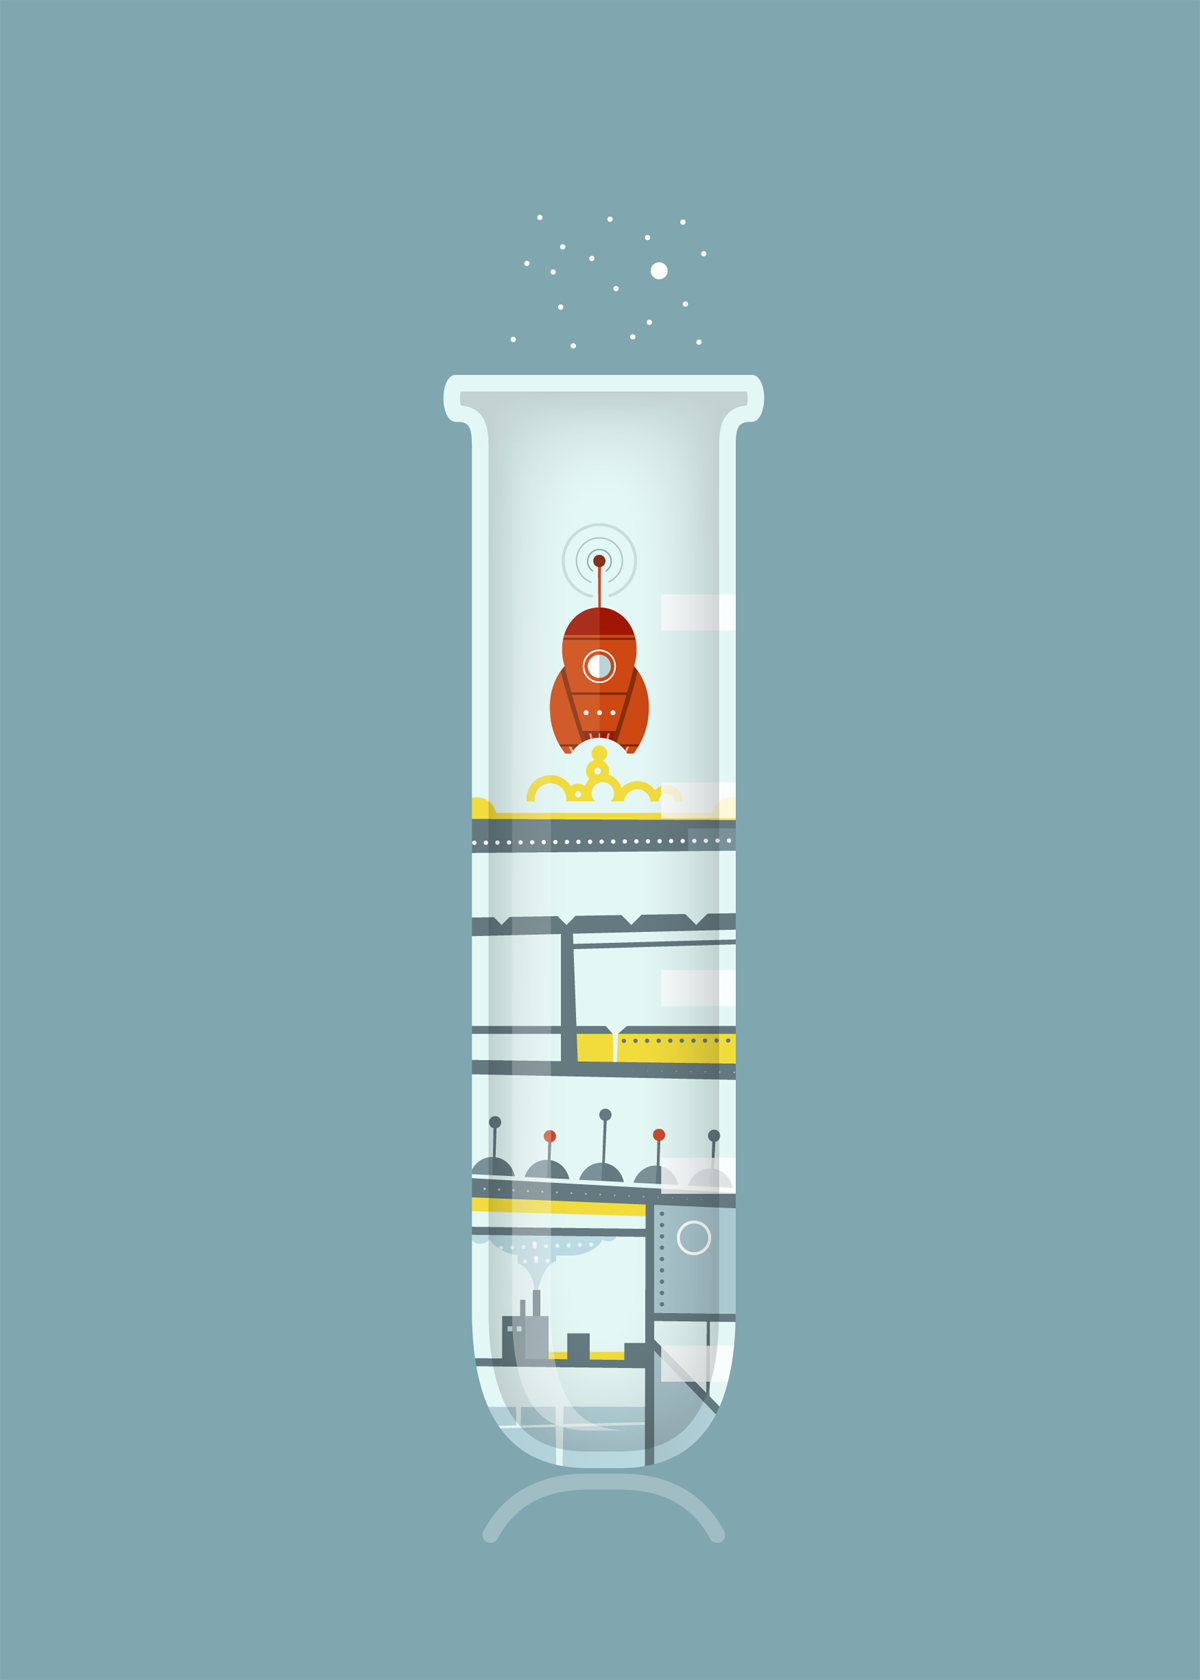
\includegraphics[width=0.42\textwidth]{endmatter/colophon.png}
\end{figure}

% If you don't want an image in the colophon:
% \vspace*{200pt}

\begin{center}
\parbox{200pt}{\lettrine[lines=3,slope=-2pt,nindent=-4pt]{\textcolor{SchoolColor}{T}}{his thesis was typeset} using \LaTeX, originally developed by Leslie Lamport and based on Donald Knuth's \TeX. The body text is set in 11 point Egenolff-Berner Garamond, a revival of Claude Garamont's humanist typeface. The above illustration, \textit{Science Experiment 02}, was created by Ben Schlitter and released under \href{http://creativecommons.org/licenses/by-nc-nd/3.0/}{\textsc{cc by-nc-nd 3.0}}. A template that can be used to format a PhD dissertation with this look \textit{\&} feel has been released under the permissive \textsc{agpl} license, and can be found online at \href{https://github.com/suchow/Dissertate}{github.com/suchow/Dissertate} or from its lead author, Jordan Suchow, at \href{mailto:suchow@post.harvard.edu}{suchow@post.harvard.edu}.}
\end{center}


\end{document}
